\documentclass{beamer}

\usepackage{xcolor}
\usepackage{minted}
\usepackage{amssymb}

\author{Jakob Zwirchmayr}
\title{Orange and its Branching Statement ($\Delta$) Analysis}
\date{\today}


\begin{document}

\maketitle



% ---=== FRAME ===--- %
\begin{frame}[fragile]
  \frametitle{Problem}

  \bigskip
  Overestimation in static WCET analysis 
  \begin{itemize}
    \item conservatism is a necessity
    \item more precise information might not be deducible 
  \end{itemize}

  \medskip
  $\Rightarrow$ {\it assume the worst case} \\

  \pause 

  \bigskip
  Alternatively, specify such behavior
  \begin{itemize}
    \item unknown configuration/parameters determined late  
  \end{itemize}

  \medskip
  $\Rightarrow$ nevertheless, {\it knowledge is held by system designer} (early)
\end{frame}
%%



% ---=== FRAME ===--- %
\begin{frame}[fragile]
  \frametitle{Automotive Industry}

  \bigskip
  Highly modular designs, ``product-families''
  \begin{itemize}
    \item heavy reuse of configurable SW/HW components
  \end{itemize}

  \medskip
  $\Rightarrow$ static WCET analysis {\it results unsatisfactory} \\

  \pause 

  \bigskip
  Expert annotations to improve WCET estimates
  \begin{itemize}
    \item huge effort (high number of possible parameters)
  \end{itemize}

  \medskip
  $\Rightarrow$ {\it which to chose} and supply? \\

  \pause 

  \bigskip
  Delta-approach helps identify parameters that are ``relevant''
\end{frame}
%%



% ---=== FRAME ===--- %
\begin{frame}[fragile]
  \frametitle{Use-case: Continental Code}

  \bigskip
  Software module, 700 locs
  \begin{itemize}
    \item 85 variables are possible configuration/parameters
    \item 30 values deemed relevant by an expert
  \end{itemize}

  \medskip
  $\Rightarrow$ improves estimate by 5.7\% \\

  \pause 

  \bigskip
  Delta identifies 10 conditions deemed relevant
  \begin{itemize}
    \item supplying values for related (``grep'') parameters (18)
  \end{itemize}

  \medskip
  $\Rightarrow$ improves estimate by 4.6\%
\end{frame}
%%



% ---=== FRAME ===--- %
\begin{frame}[fragile]
  \frametitle{Principles}
  \bigskip
  Bottom-up computation and propagation of node weights
  \begin{itemize}
    \item comparable to tree based WCET computation
    \item on internal representation of oRange
  \end{itemize}

  \pause 

  \bigskip
  For branching statements
  \begin{itemize}
    \item delta = difference between alternatives
  \end{itemize}

  \medskip
  {\it high delta} $\Rightarrow$ {\it high impact} on WCET estimate
\end{frame}
%%



% ---=== FRAME ===--- %
\begin{frame}[fragile]
  \frametitle{Goal \& Overview}

  \bigskip
  Unspecified behaviour due to 
  \begin{itemize}
    \item SW modularity, HW configuration or parameter variables
  \end{itemize}

  \pause

  \bigskip
  Global WCET {\it too coarse}. {\it Delta analysis} helps identify 
  \begin{itemize}
    \item \textcolor{red}{\bf relevant} configuration/parameter variables
  \end{itemize}
  that {\it likely impact the WCET}.
\end{frame} 
%%



% ---=== FRAME ===--- %
\begin{frame}[fragile]
  \frametitle{Illustration}

  \begin{itemize}
    \item {\tt cheap()} v.s.~{\tt cheap()} \textcolor{green}{\Large \checkmark}
    \item {\tt 2*expensive()} v.s.~{\tt 2*expensive()}: \textcolor{green}{\Large \checkmark}
    \item {\tt 2*expensive()} v.s.~{\tt expensive()}: \textcolor{red}{\bf !! \small \tt (param4)}
  \end{itemize}

  \begin{figure}
    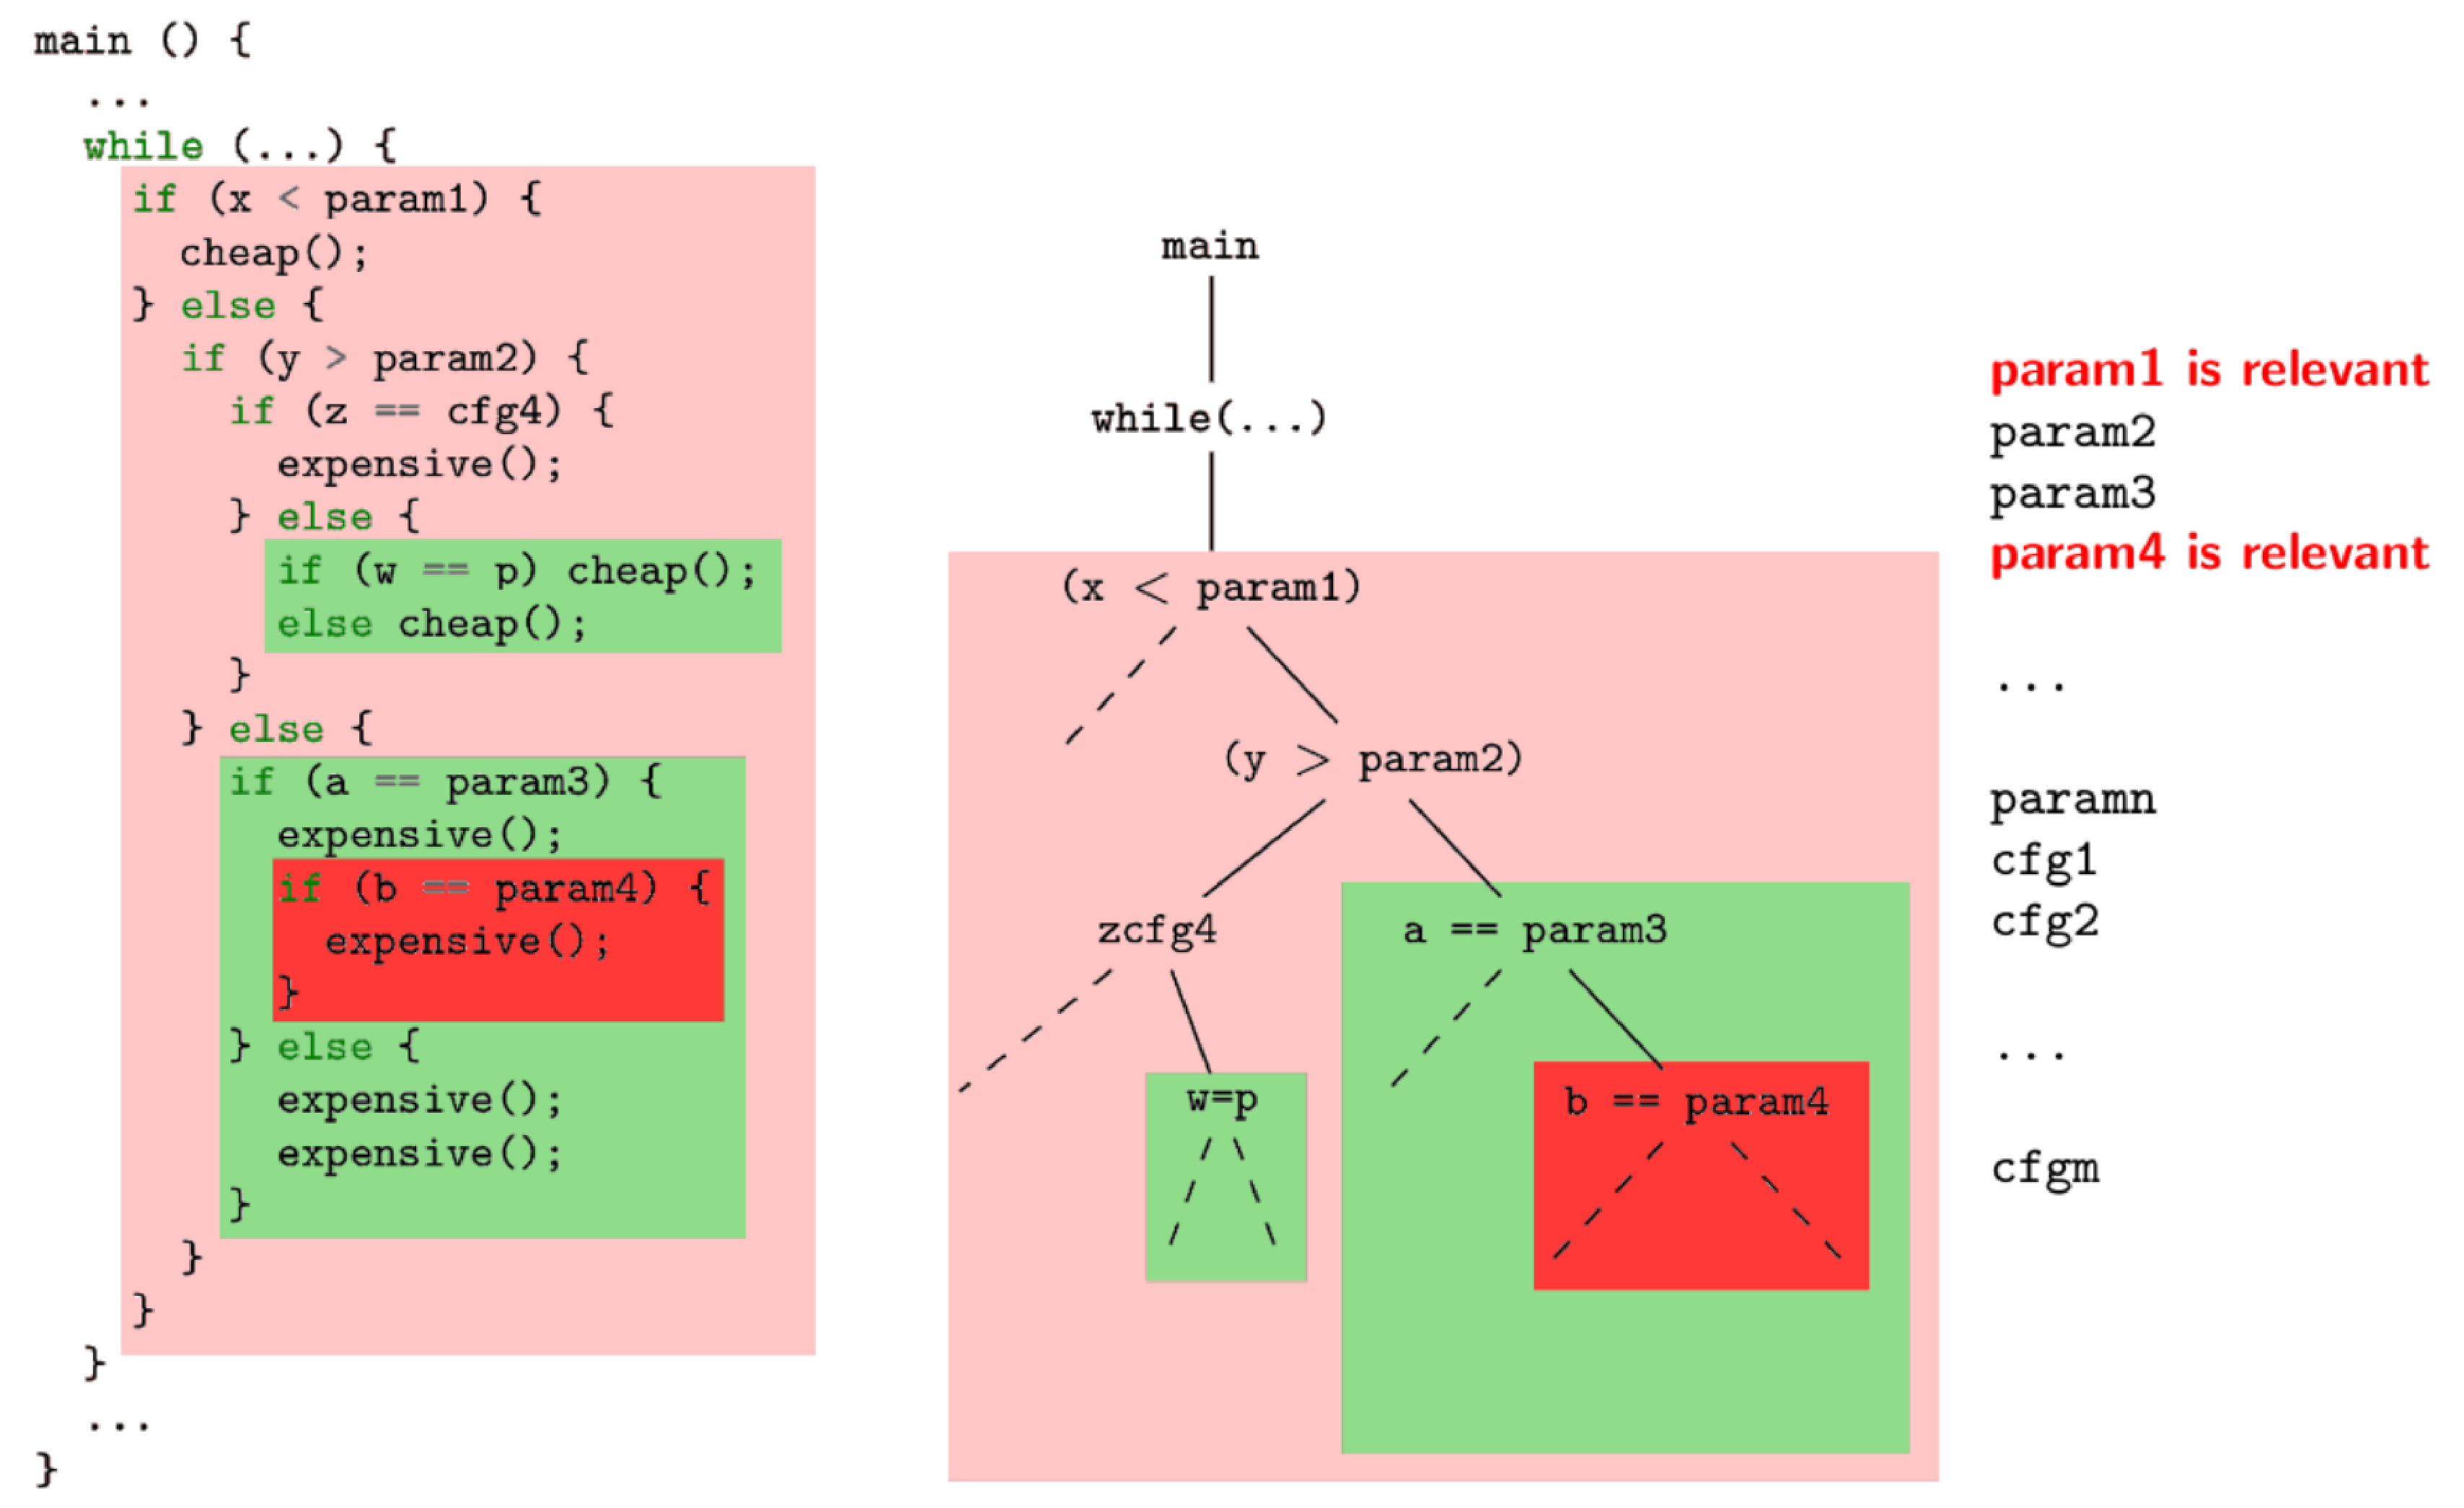
\includegraphics[width=10cm]{img/overview.pdf} 
  \end{figure}
\end{frame} 
%%



% ---=== FRAME ===--- %
\begin{frame}[fragile]
  \frametitle{Outlook, Future Work}

  \bigskip
  Cost model 
  \begin{itemize}
    \item means of early ``WCET analysis'' in design (unsafe!)
  \end{itemize}

  \bigskip
  Combine with program analysis 
  \begin{itemize}
    \item identify where it pays off to invest analysis effort
  \end{itemize}

  \bigskip
  Improve usability and specification effort 
  \begin{itemize}
    \item ``eclipse'' support
    \item alternative delta-orderings, highlighting
    \item means to input value annotations
  \end{itemize}
\end{frame}
%%



% ---=== FRAME ===--- %
\begin{frame}[fragile]
  \frametitle{}

  \begin{center}
  Hands-on oRange and Delta Analysis
  \end{center}
\end{frame} 
%%



% ---=== FRAME ===--- %
\begin{frame}[fragile]
  \frametitle{Orange Overview}

  \bigskip 
  Flow-analysis
  \begin{itemize}
    \item on source-level
  \end{itemize}

  \bigskip
  Main objective 
  \begin{itemize}
    \item loop bound analysis
  \end{itemize}

  \bigskip
  Additionally 
  \begin{itemize}
    \item infeasible paths analysis
  \end{itemize}

  \bigskip
  Based on 
  \begin{itemize}
    \item abstract interpretation 
  \end{itemize}
\end{frame} 
%%



% ---=== FRAME ===--- %
\begin{frame}[fragile]
  \frametitle{Orange Usage Dialog}
  \begin{center}
    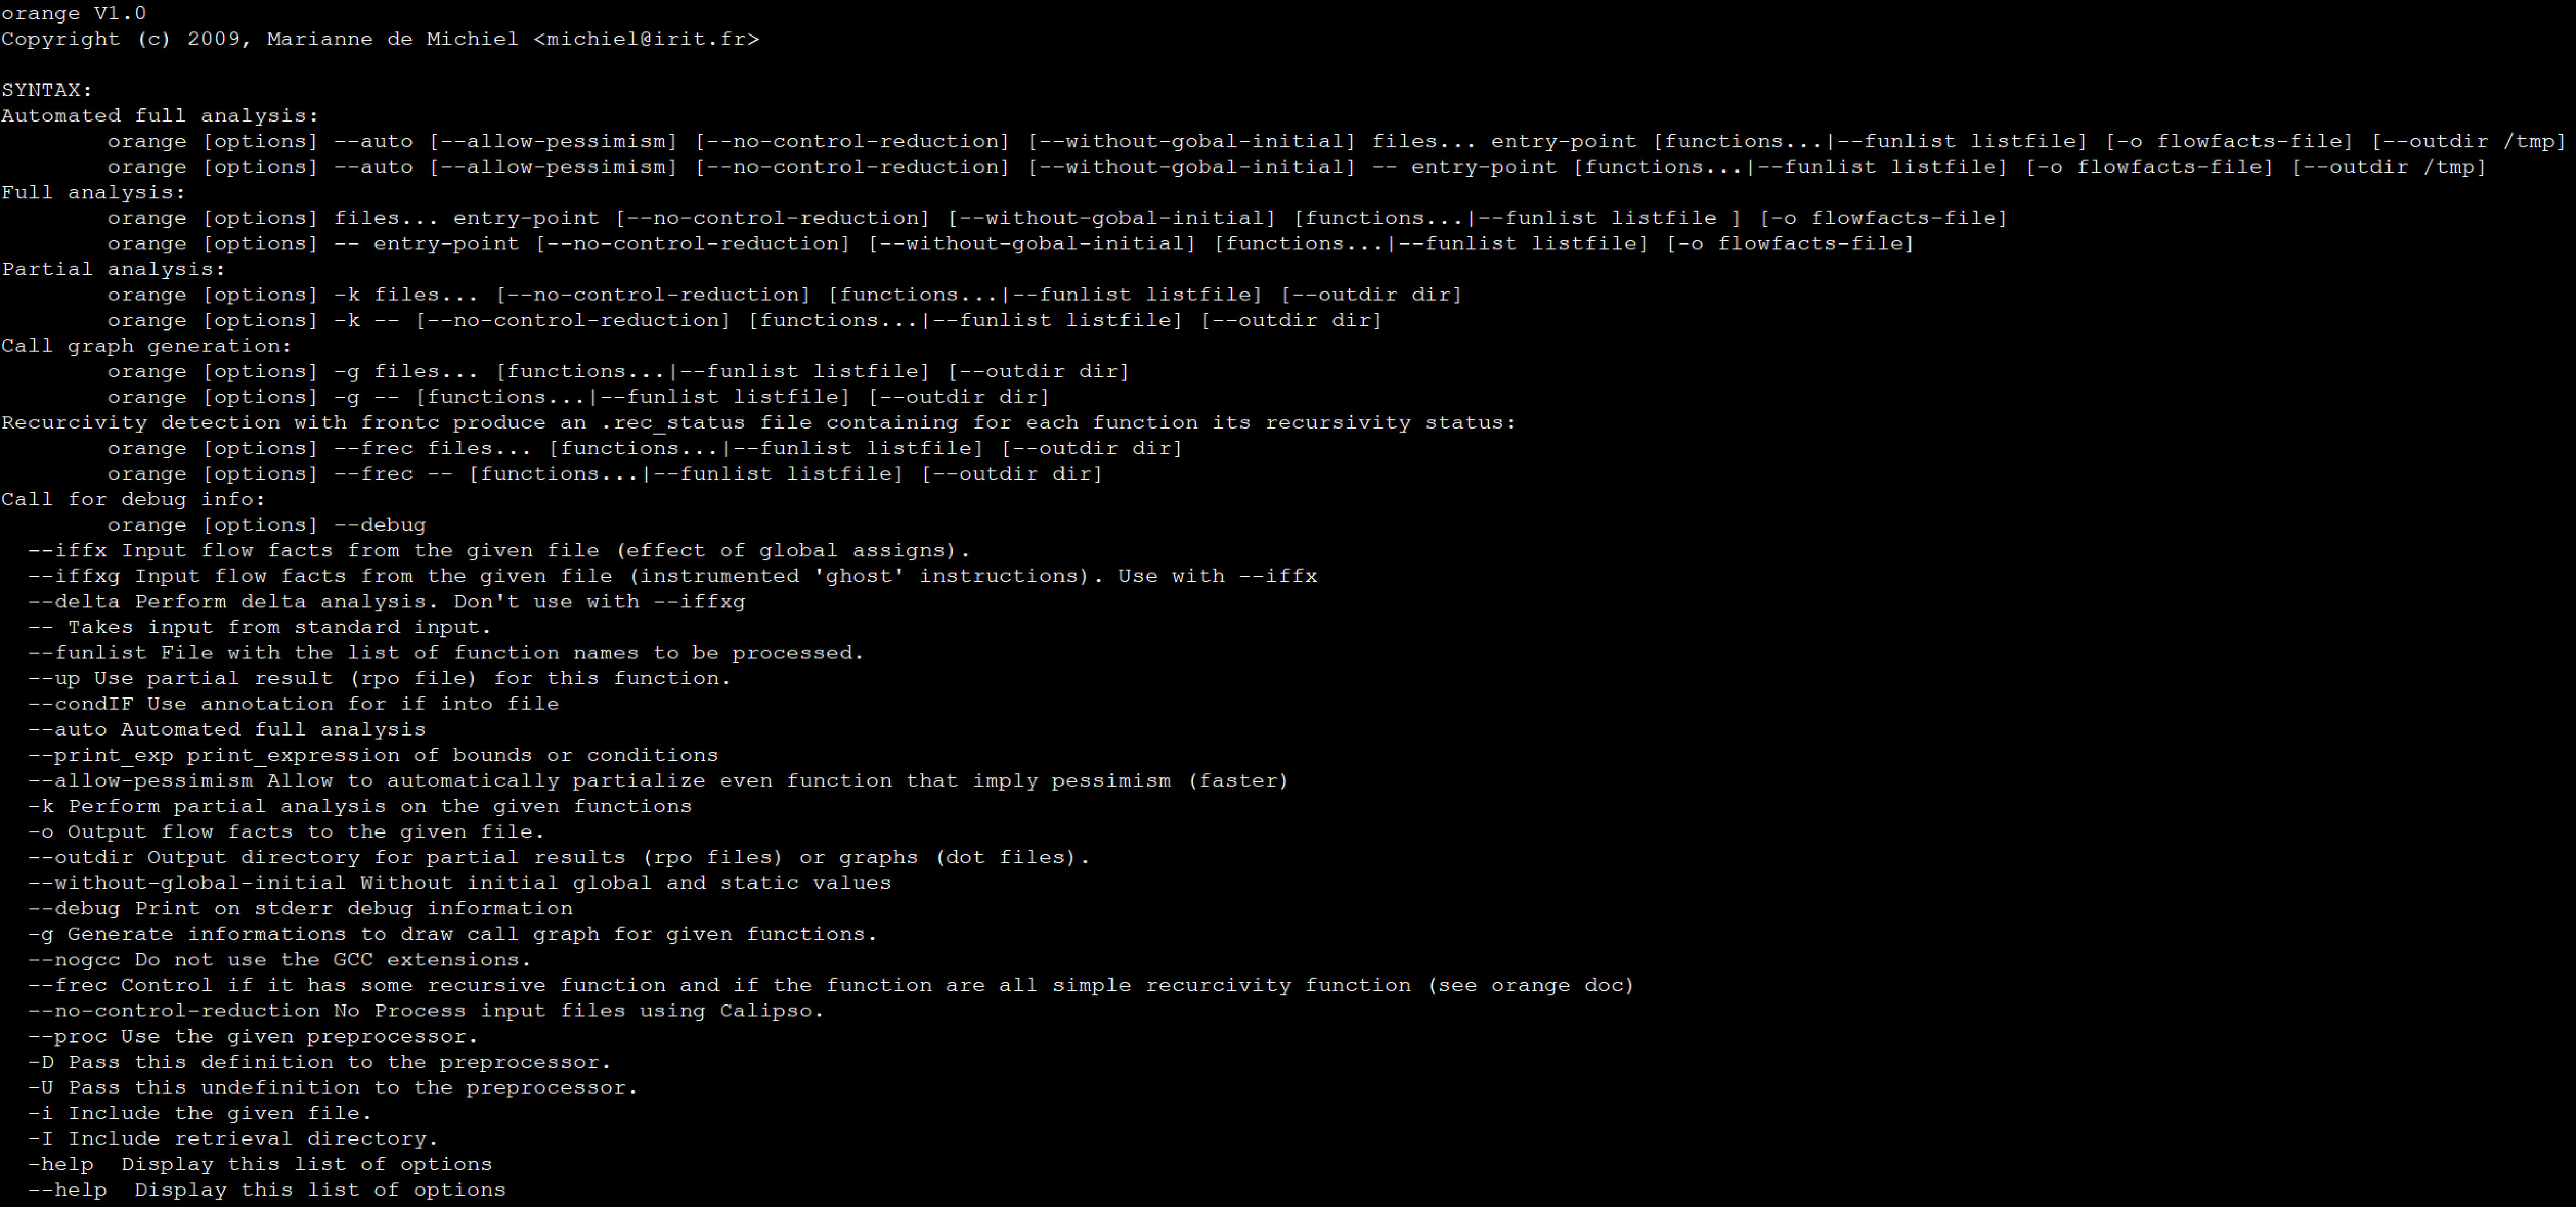
\includegraphics[width=11cm]{img/orange_flags.pdf} \\

    \bigskip
    Orange flags.
  \end{center}
\end{frame} 
%%



% ---=== FRAME ===--- %
\begin{frame}[fragile]
  \frametitle{Nonsensical Running Example}
  {\tiny
  \begin{minipage}[t]{0.35\textwidth}
    \begin{minted}{c}
void main () {
  int i, j, k, l, m, n, o, x,y,z;

  if (i) i = i * 2 + 1;
  else i--;

  for (j = 0; j < 10; j++)
    k += i;

  if (k > 0) {
    k = k * 2 - 1;
    l = k * 2 + 1;

    if (l > 100) {
      m = l;
      if (x) 
        if (y)
          if (z) ;
          else ;
        else ;
      else ;
      n = 0;
      i = 0;
    } else {
      i = 100;
      n = 100;
    } 

    if (n == 0 && k == 5) n++;
    else {
      n = 2 * n + 1;
      m = k;
    }
    o = n + k + m;
  } else 
    \end{minted}
  \end{minipage}
  }
  \begin{minipage}[t]{0.6\textwidth}
    {\tiny
    \begin{minted}{c}
  ... 
  } else 
      k = 0;
  if (k == 0) {
    i = 2 * i + 1;
    j = k * 3 - 1;
    k = m / 2 + i;
    l = -n;
    o = j * 2 - n;
    i = l + o;
    o = i + j + k + l + o + i; 
  } else 
      i = 0;
}
    \end{minted}
    }

    \bigskip
    \begin{centering}
      Analyze {\tt main} function in file {\tt rex.c}: \\
      {\small
      \begin{minted}{sh}
        > ./orange rex.c main
      \end{minted}
      }
    \end{centering}
  \end{minipage}
\end{frame} 
%%



% ---=== FRAME ===--- %
\begin{frame}[fragile]
  \frametitle{Standard Orange Output}

  \begin{center}
    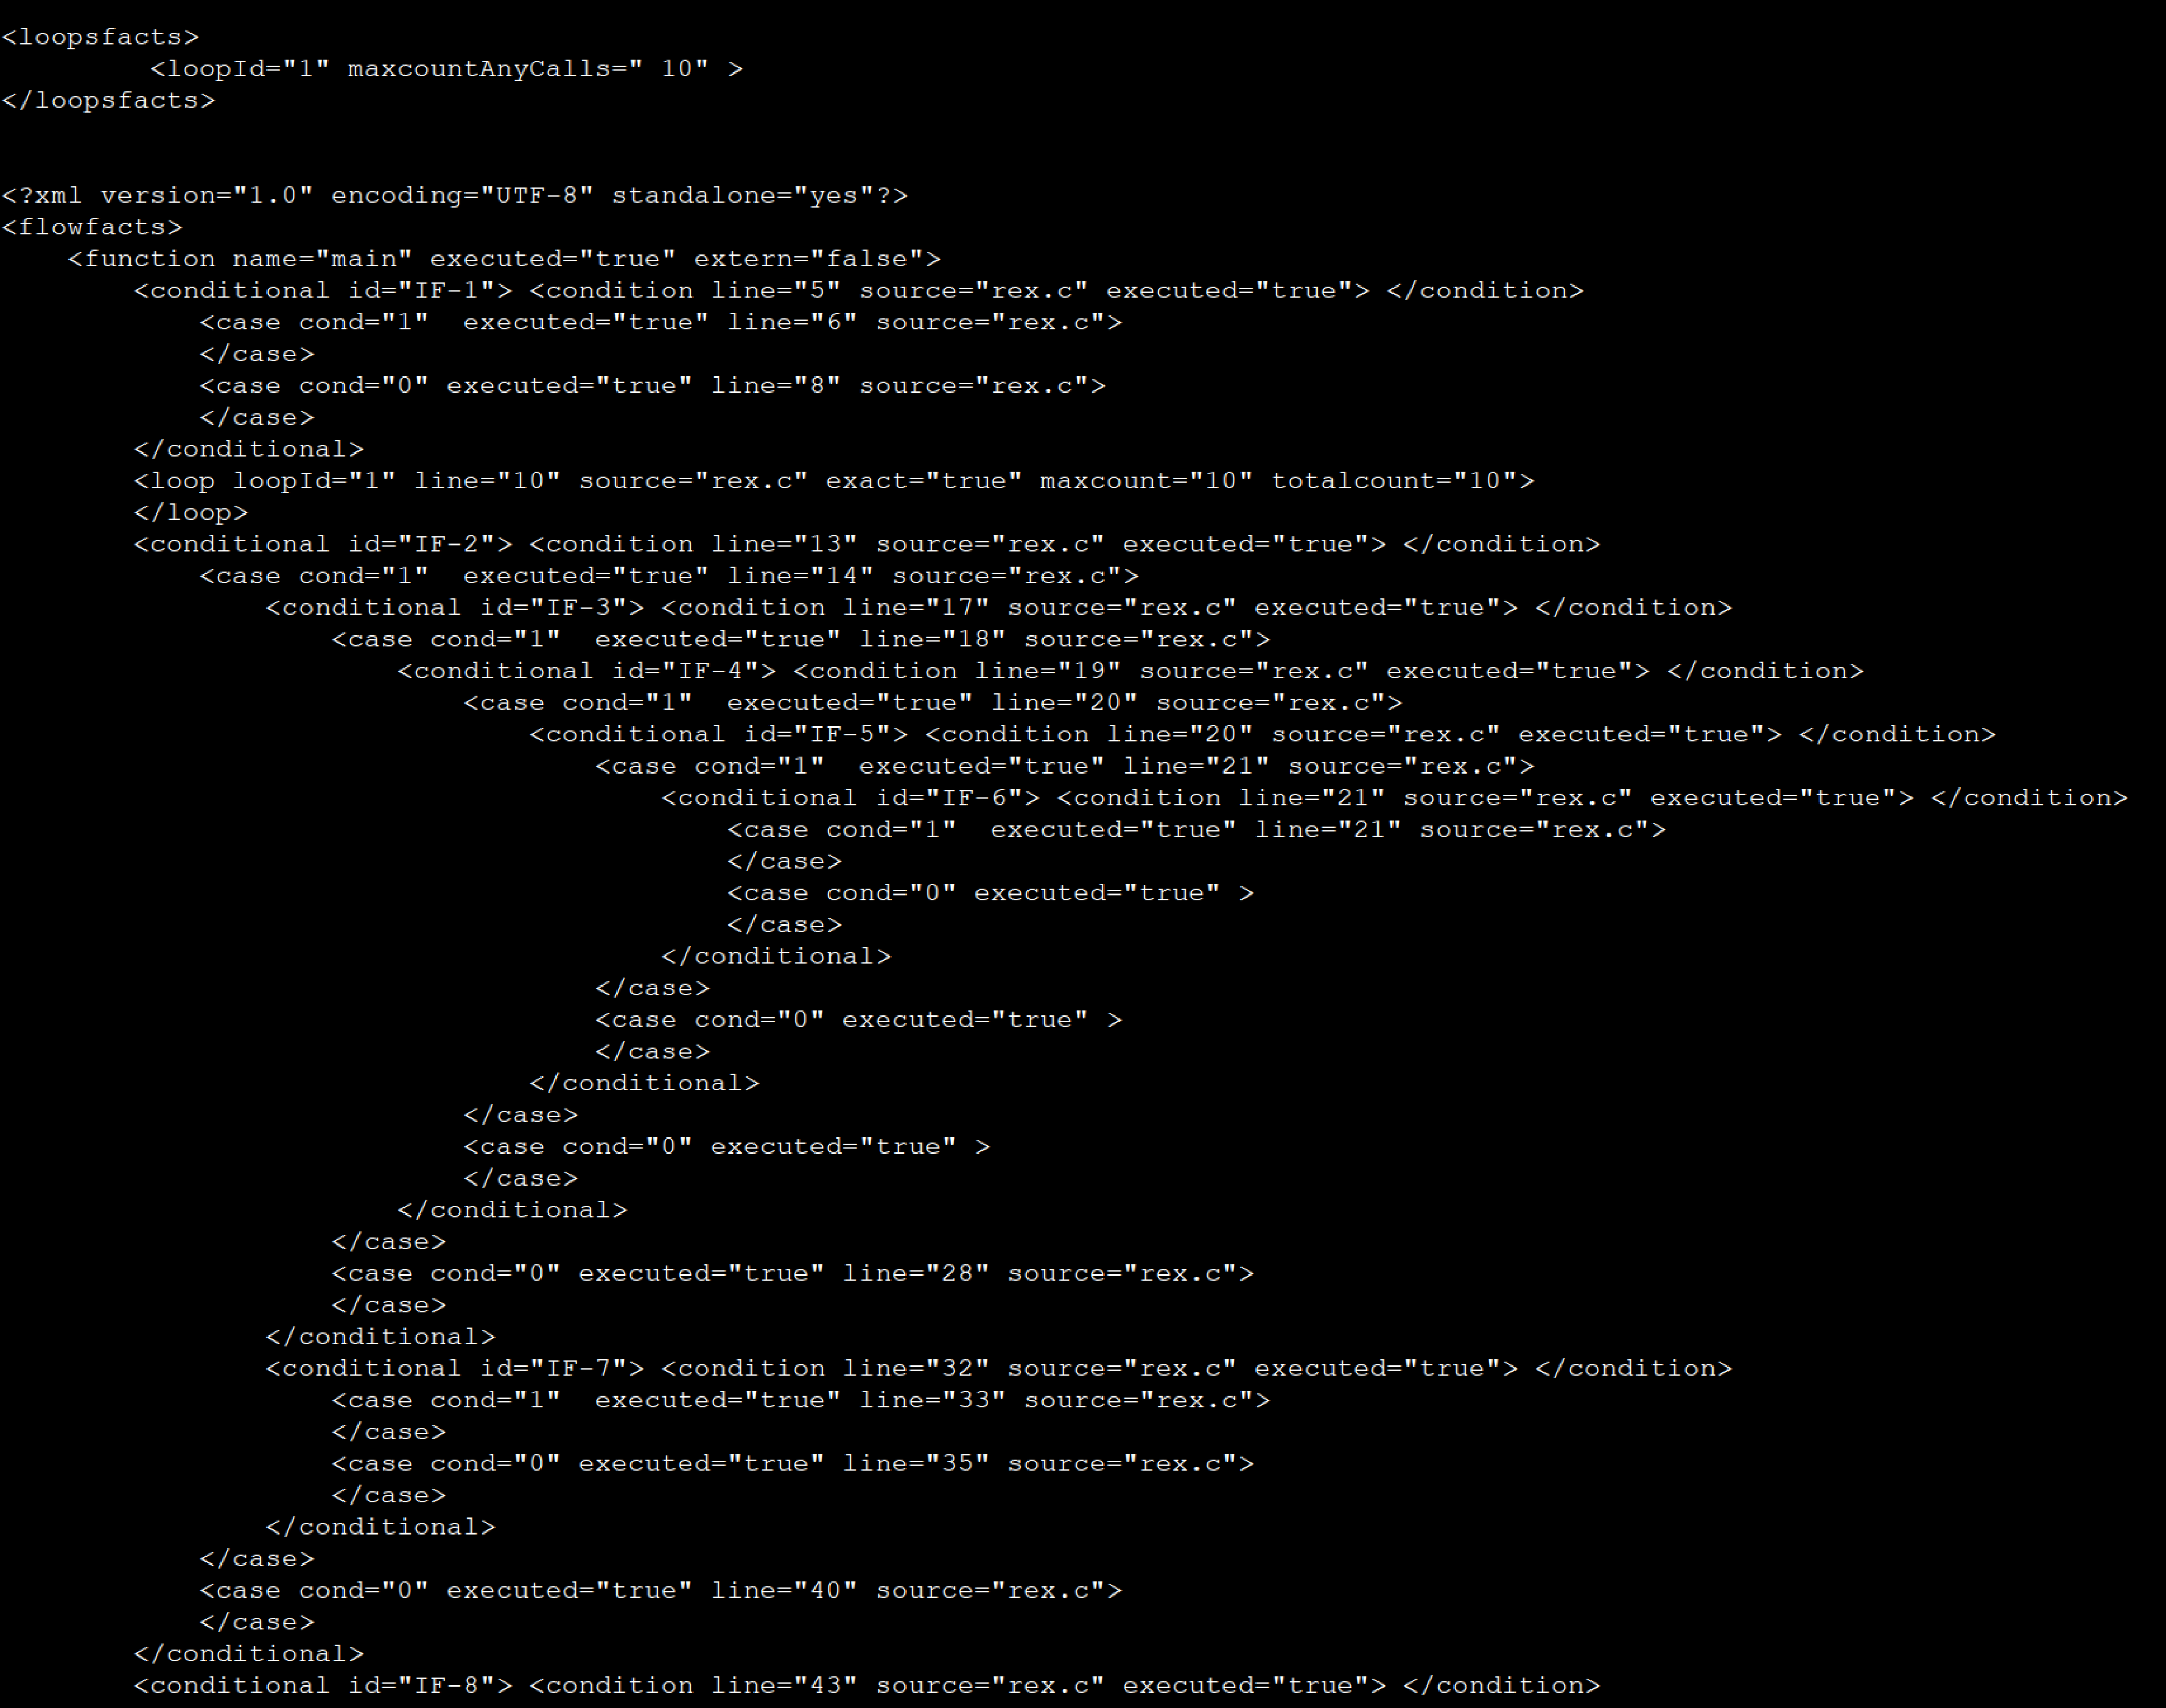
\includegraphics[width=9cm]{img/std_orange_out.pdf} \\
     Loopfacts and FFX. 
  \end{center}
\end{frame} 
%%



% ---=== FRAME ===--- %
\begin{frame}[fragile]
  \frametitle{Orange Output: FFX}

  \begin{center}
    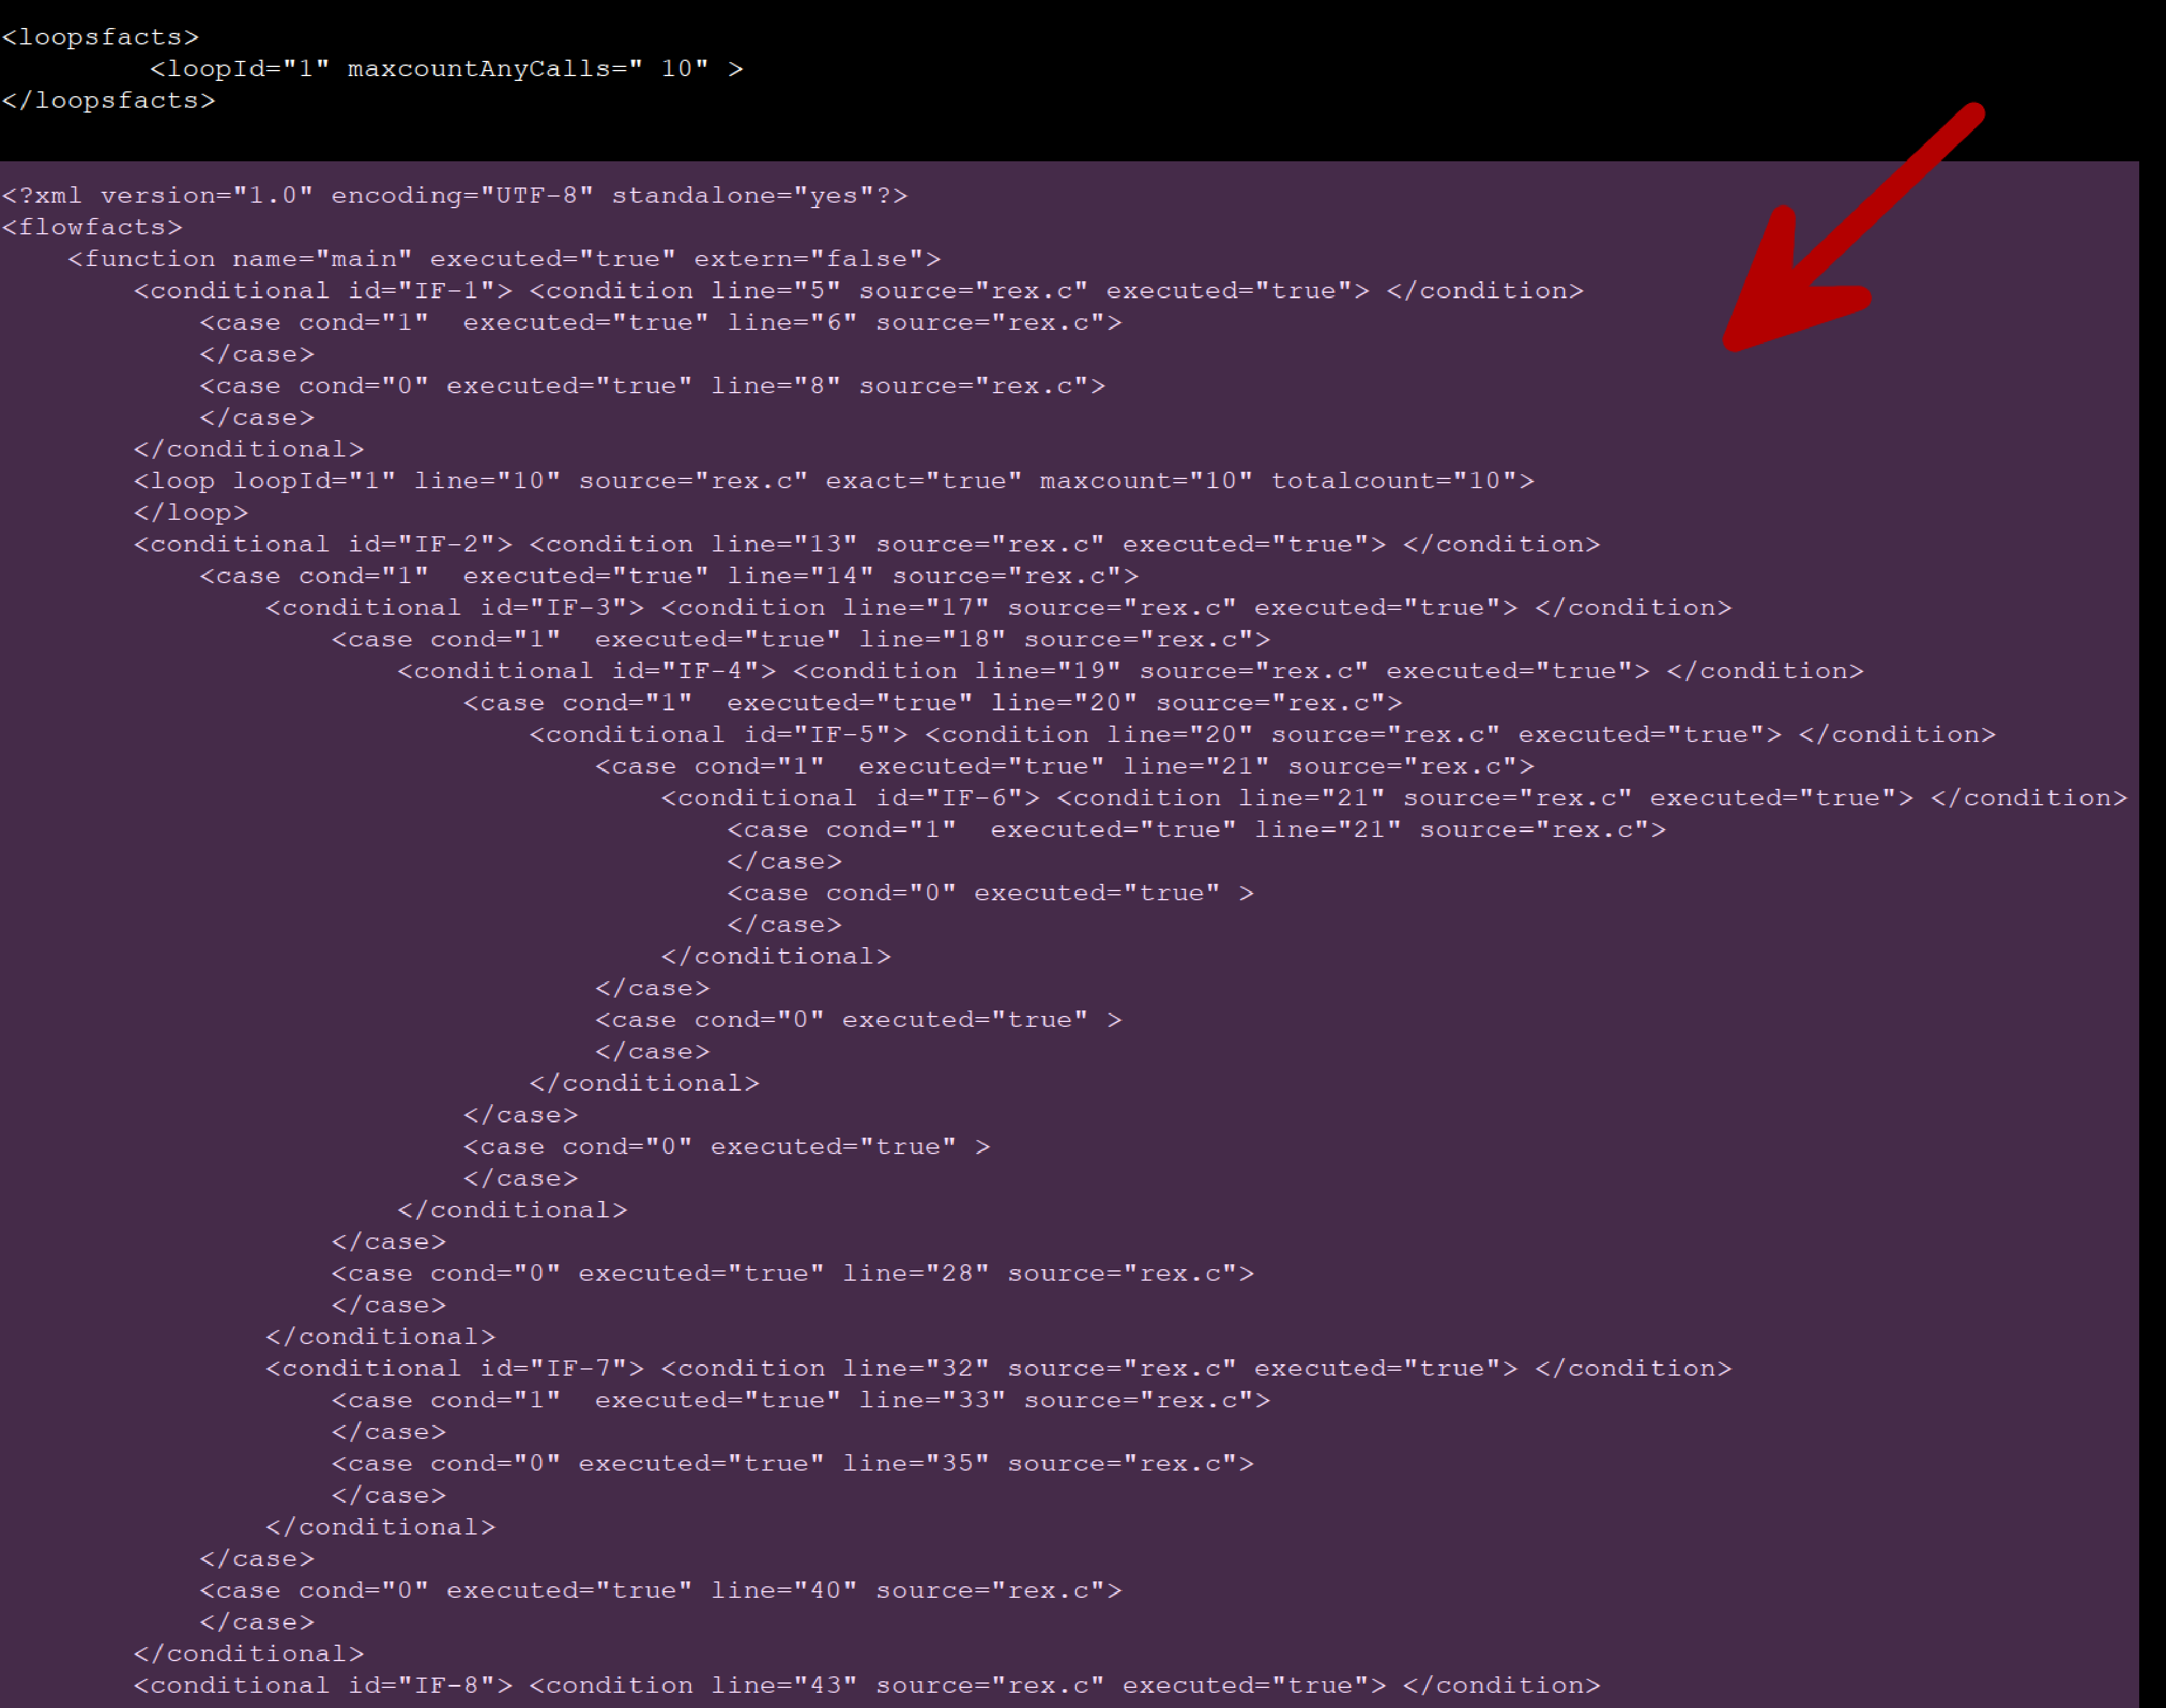
\includegraphics[width=9cm]{img/the_ffx.pdf} \\
    Flowfacts: calls inlined, contextual information.
  \end{center}
\end{frame} 
%%



% ---=== FRAME ===--- %
\begin{frame}[fragile]
  \frametitle{FFX}

  \medskip
  Flowfacts
  \begin{itemize}
    \item XML based
  \end{itemize}

  \medskip
  Elements (tags)
  \begin{itemize}
    \item represent statements
  \end{itemize}

  \medskip
  Attributes
  \begin{itemize}
    \item carry analysis (and location) information, e.g.~
    \item {\tt max/totalcount} (loops) and {\tt executed} (conditions)
  \end{itemize}

  \medskip
  ``Call-graph''
  \begin{itemize}
    \item calls are ``inlined''
  \end{itemize}
\end{frame} 
%%



% ---=== FRAME ===--- %
\begin{frame}[fragile]
  \frametitle{Orange Output: Loopfacts}

  \begin{center}
    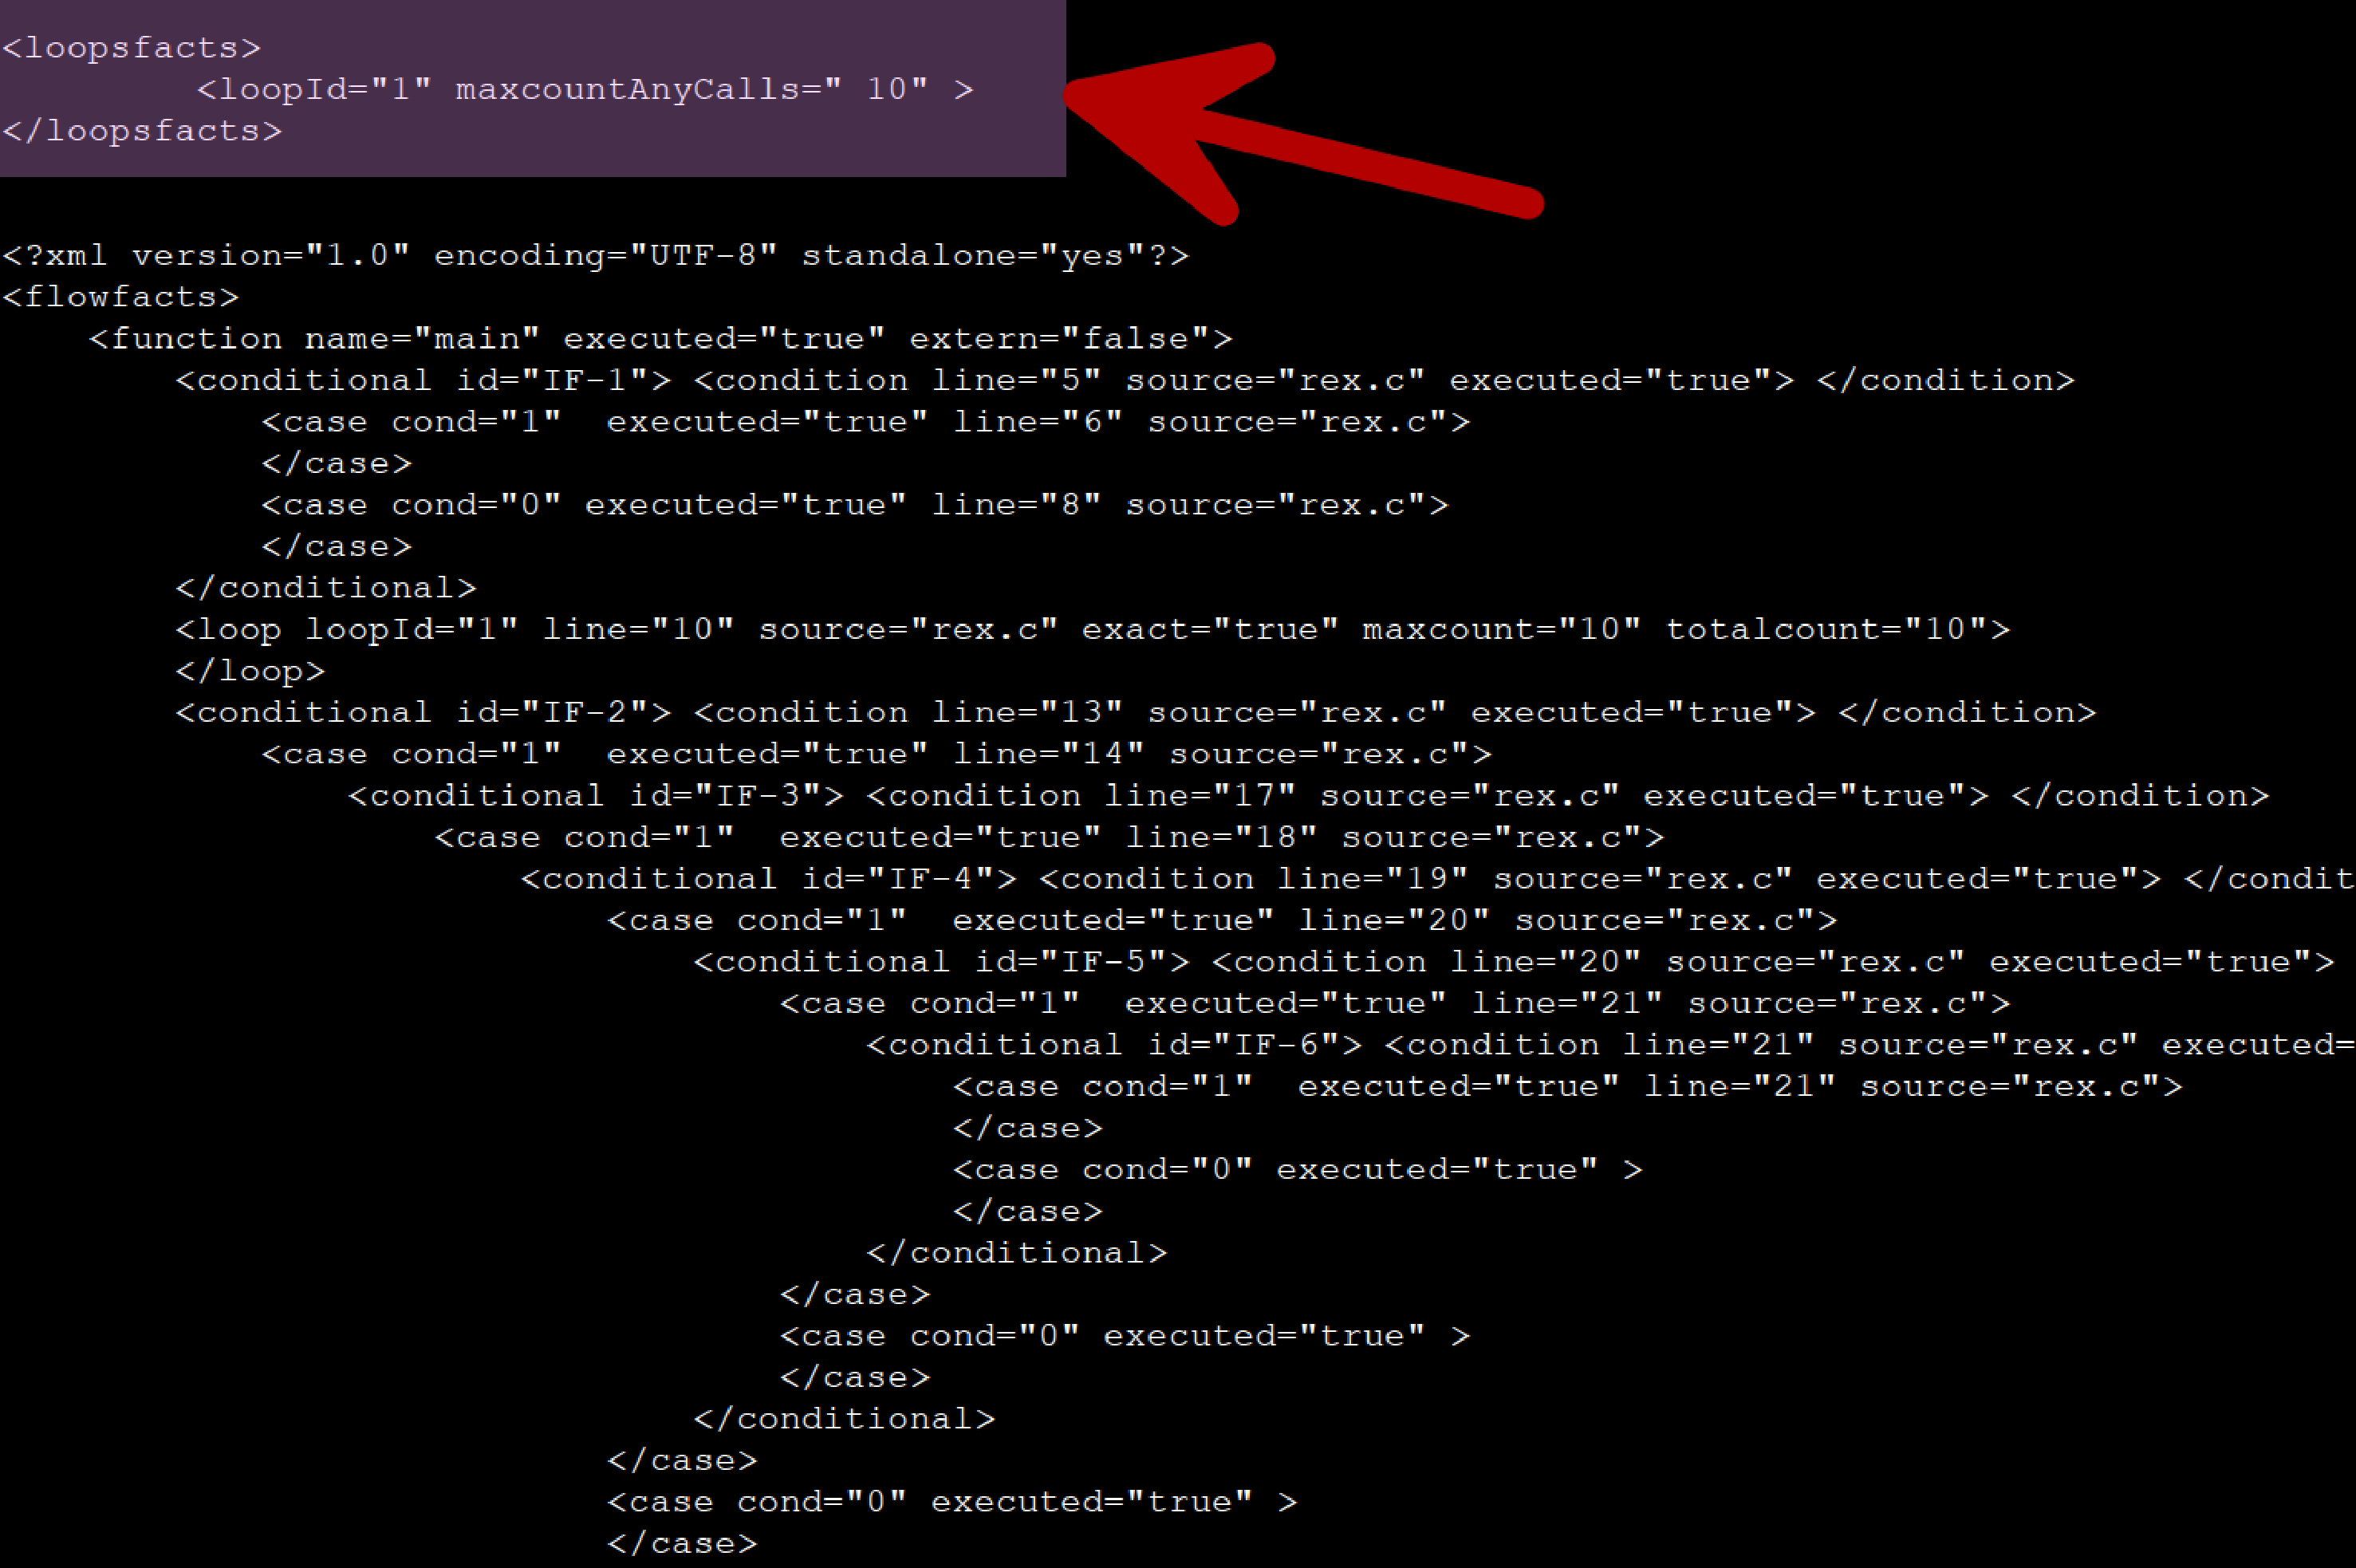
\includegraphics[width=9cm]{img/loopsfacts.pdf} \\
    Loopfacts: valid over all executions.
  \end{center}
\end{frame} 
%%



% ---=== FRAME ===--- %
\begin{frame}[fragile]
  \frametitle{Loopfacts}

  \medskip
  Recall, FFX ``call-graph'' structure
  \begin{itemize}
     \item models (to some extent) the structure of the program
  \end{itemize}

  \medskip
  Thus, flowfacts are 
  \begin{itemize}
    \item contextual
    \item valid in relation to ``surrounding'' \textcolor{red}{CHECK!} call site
  \end{itemize}

  \medskip
  Loop facts are
  \begin{itemize}
    \item an exception
    \item ``maximum bound over all calls''
  \end{itemize}
\end{frame} 
%%



% ---=== FRAME ===--- %
\begin{frame}[fragile]
  \frametitle{Orange: Performing Delta Analysis}

  \begin{centering}
    Delta analyze {\tt main} function in file {\tt rex.c}: \\
    {\small
    \begin{minted}{sh}
              > ./orange rex.c main --delta
    \end{minted}
    }
  \end{centering}
\end{frame} 
%%



% ---=== FRAME ===--- %
\begin{frame}[fragile]
  \frametitle{Delta Output}

  \begin{center}
    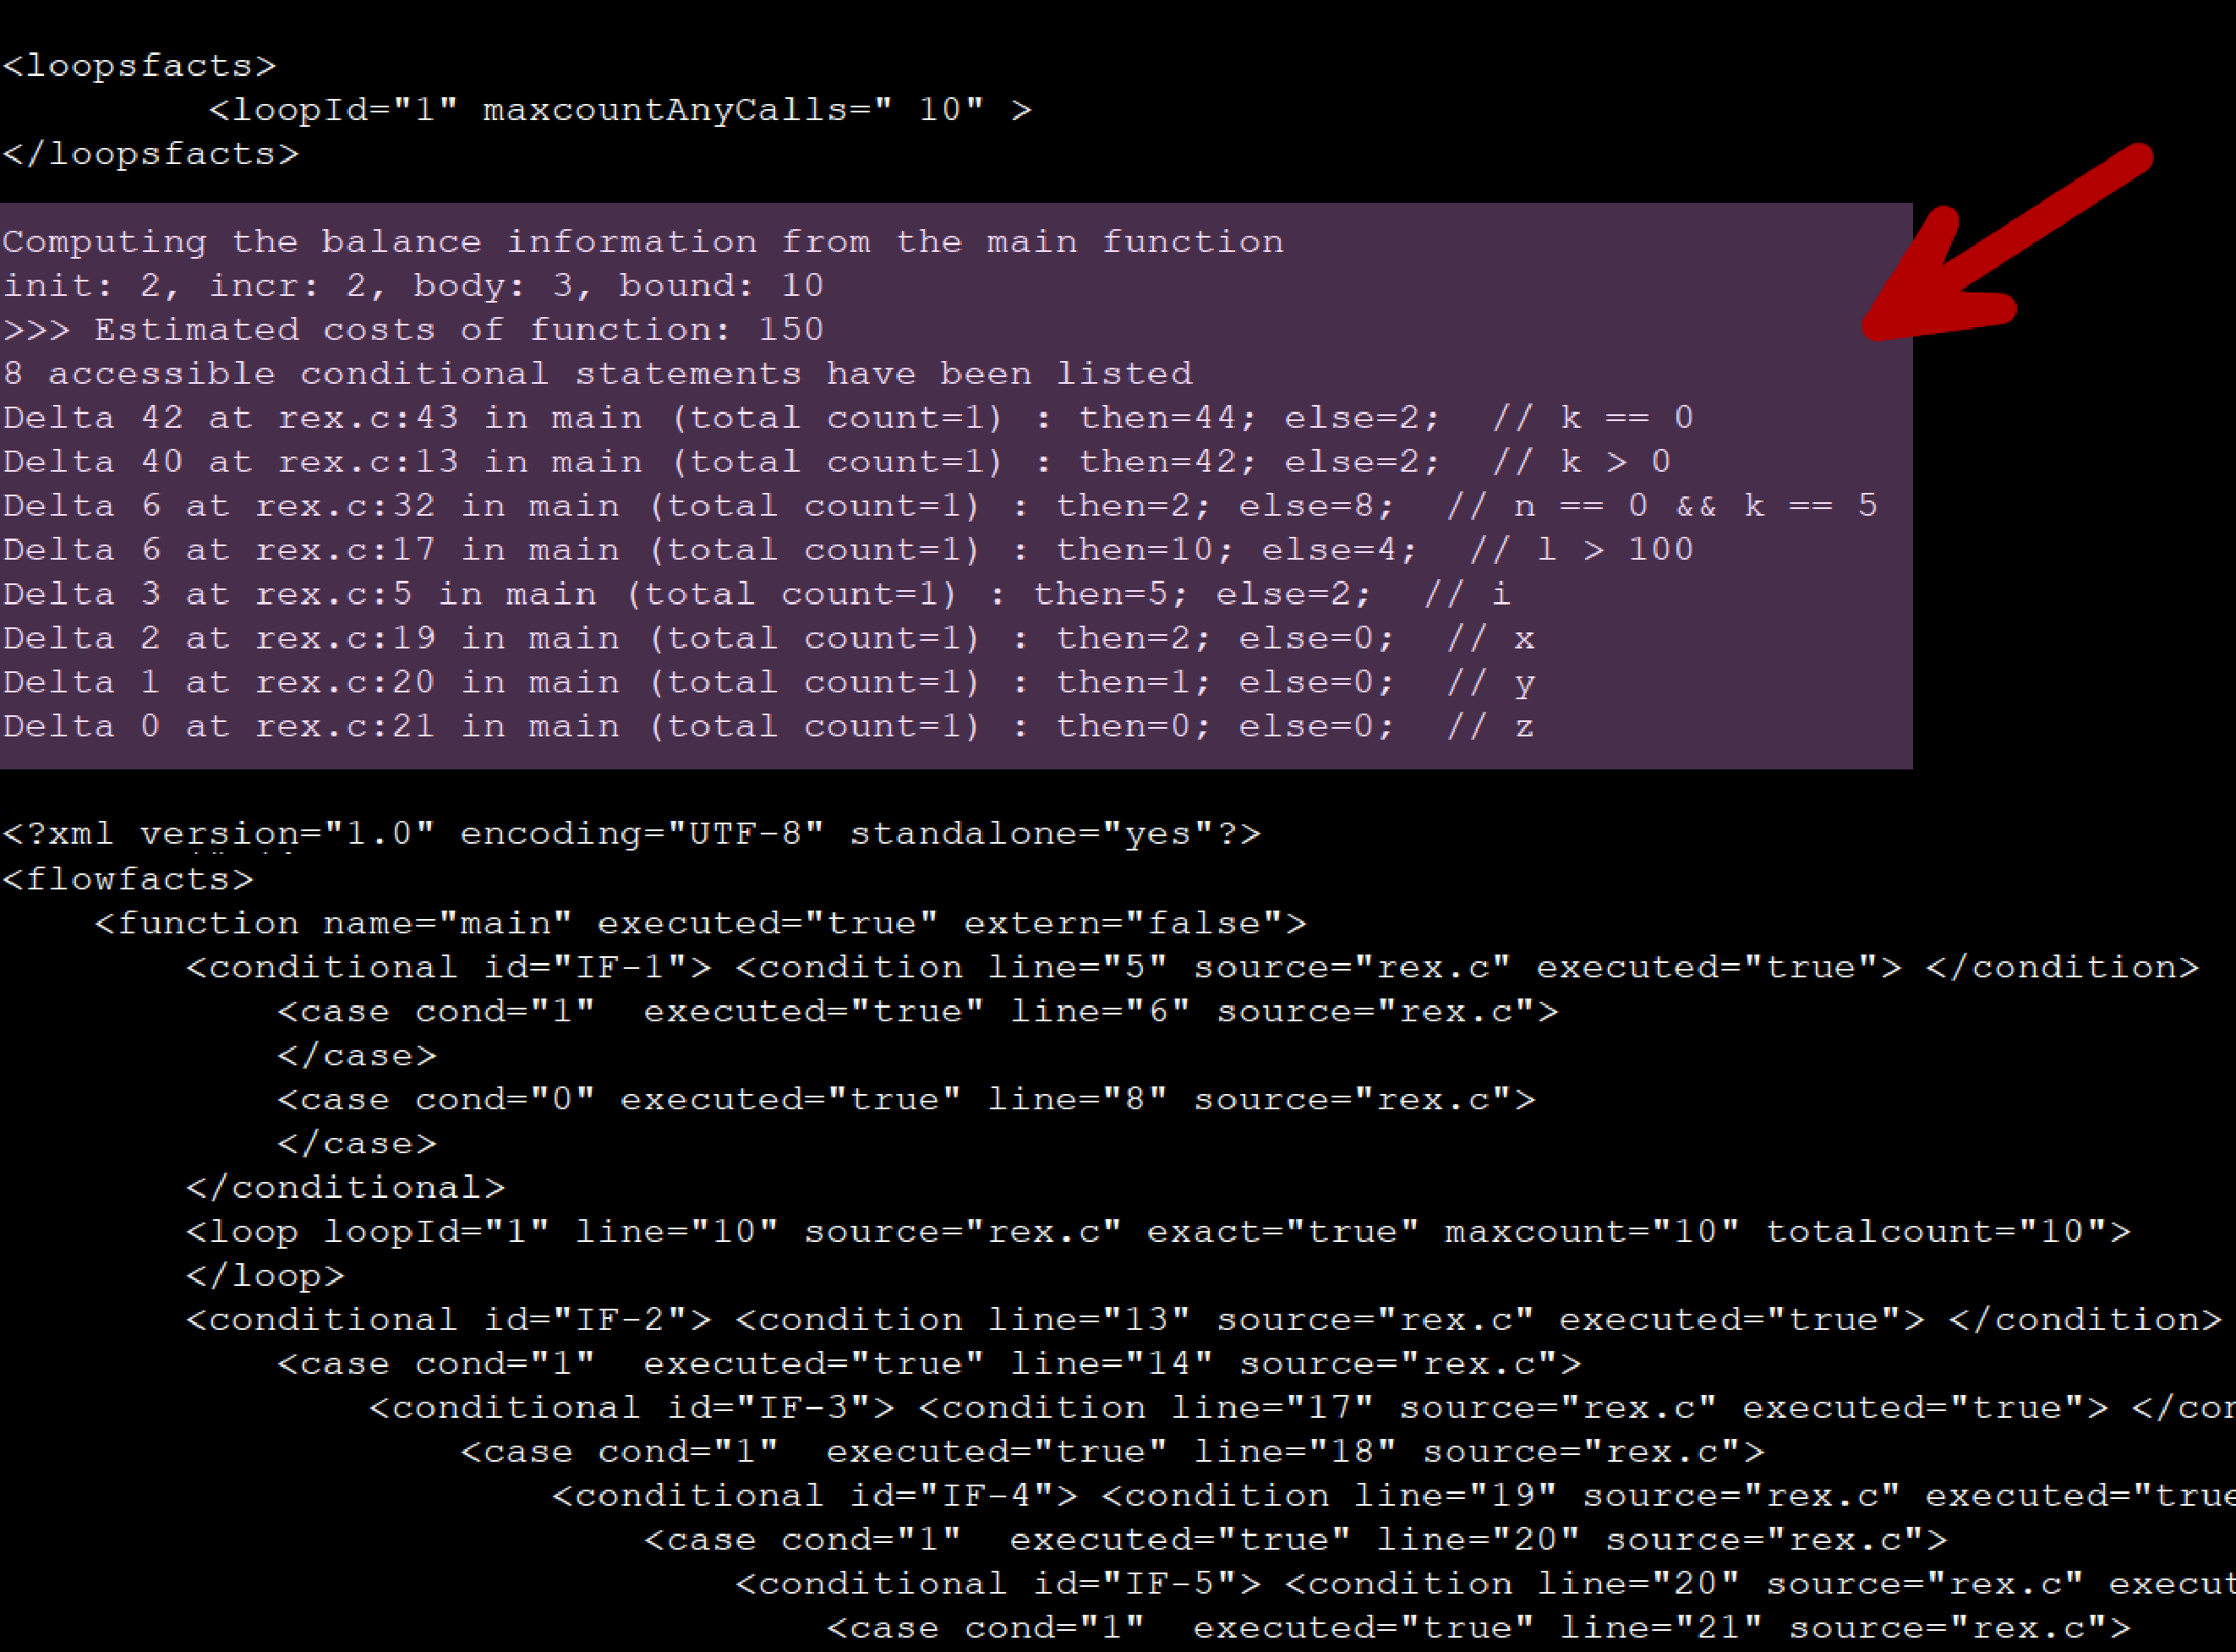
\includegraphics[width=9cm]{img/delta_output_all.pdf} \\

    \bigskip
    Output of orange when running delta-analysis.
  \end{center}
\end{frame} 
%%



% ---=== FRAME ===--- %
\begin{frame}[fragile]
  \frametitle{Delta Output: Function Costs}

  \begin{center}
    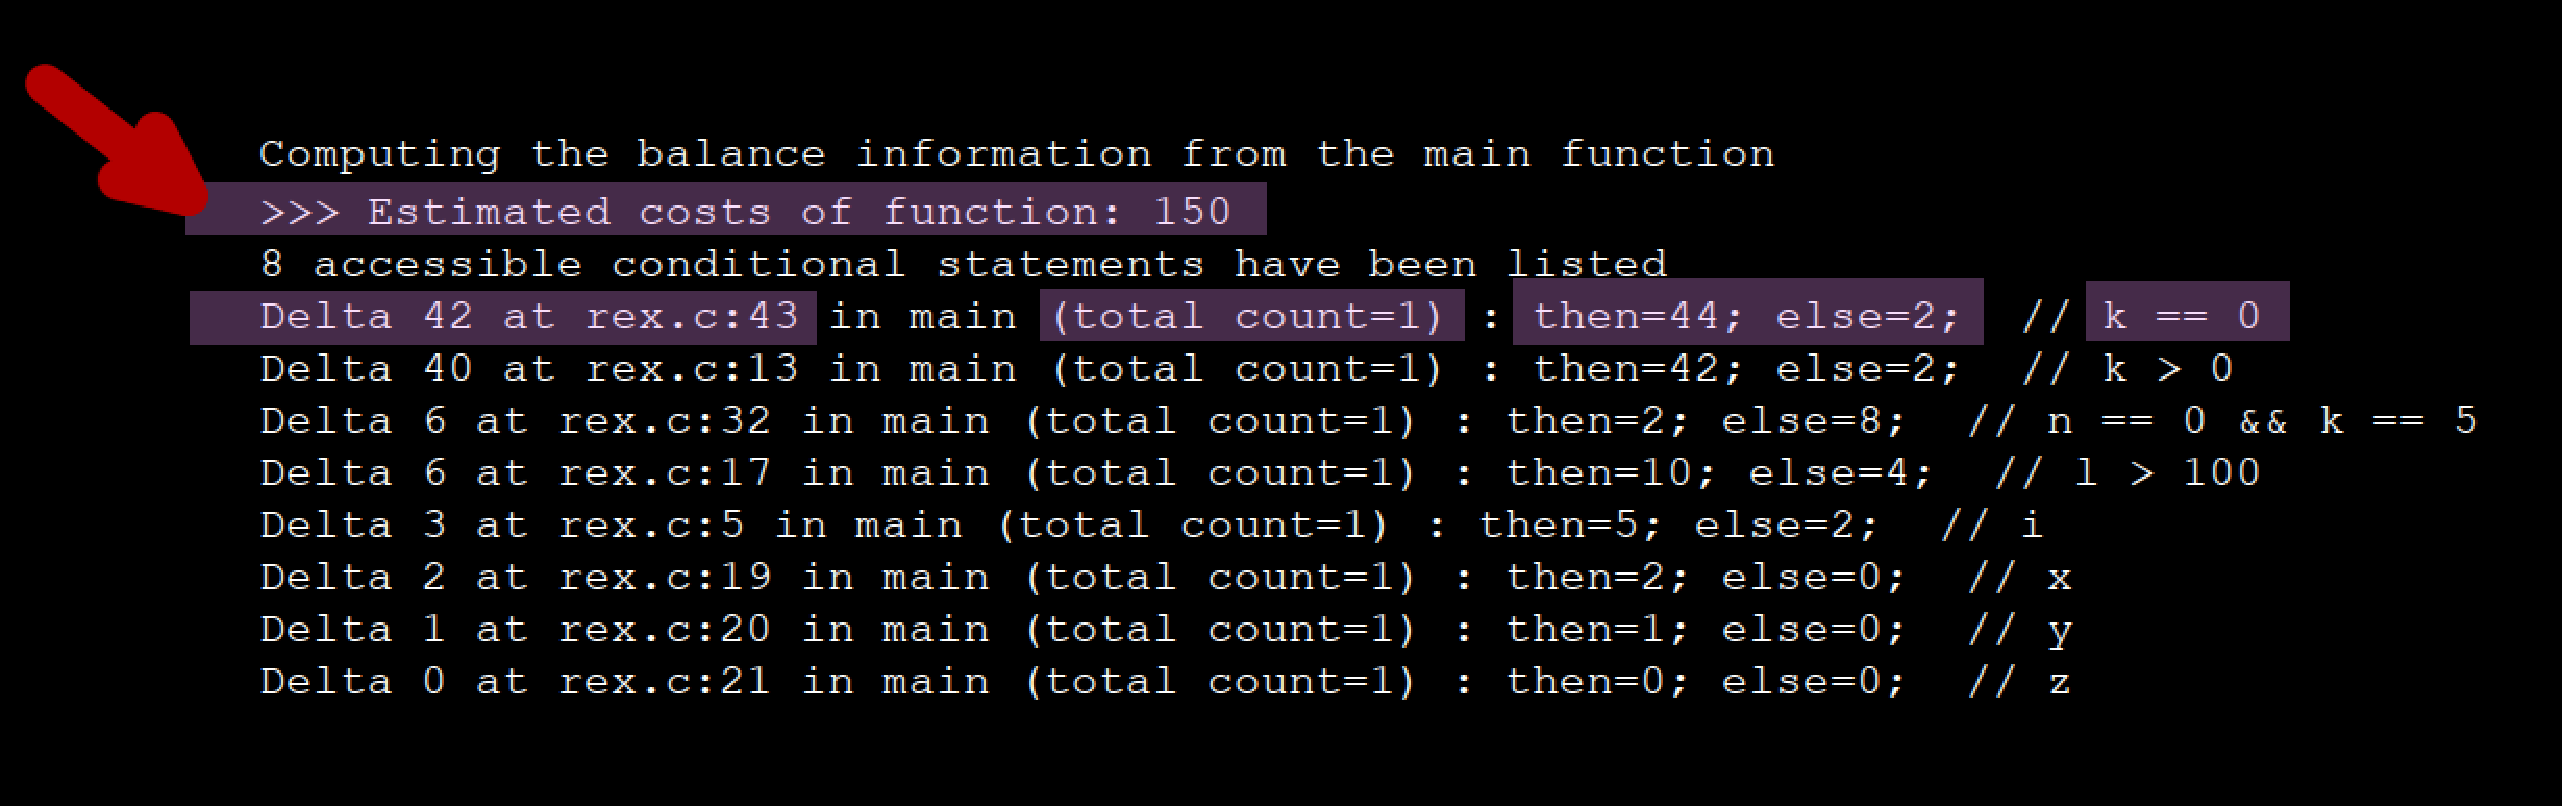
\includegraphics[width=9cm]{img/dd1.pdf} \\

    \bigskip
    Delta-analysis outputs costs of analyzed function.
  \end{center}
\end{frame} 
%%



% ---=== FRAME ===--- %
\begin{frame}[fragile]
  \frametitle{Delta Output: Delta-weight}

  \begin{center}
    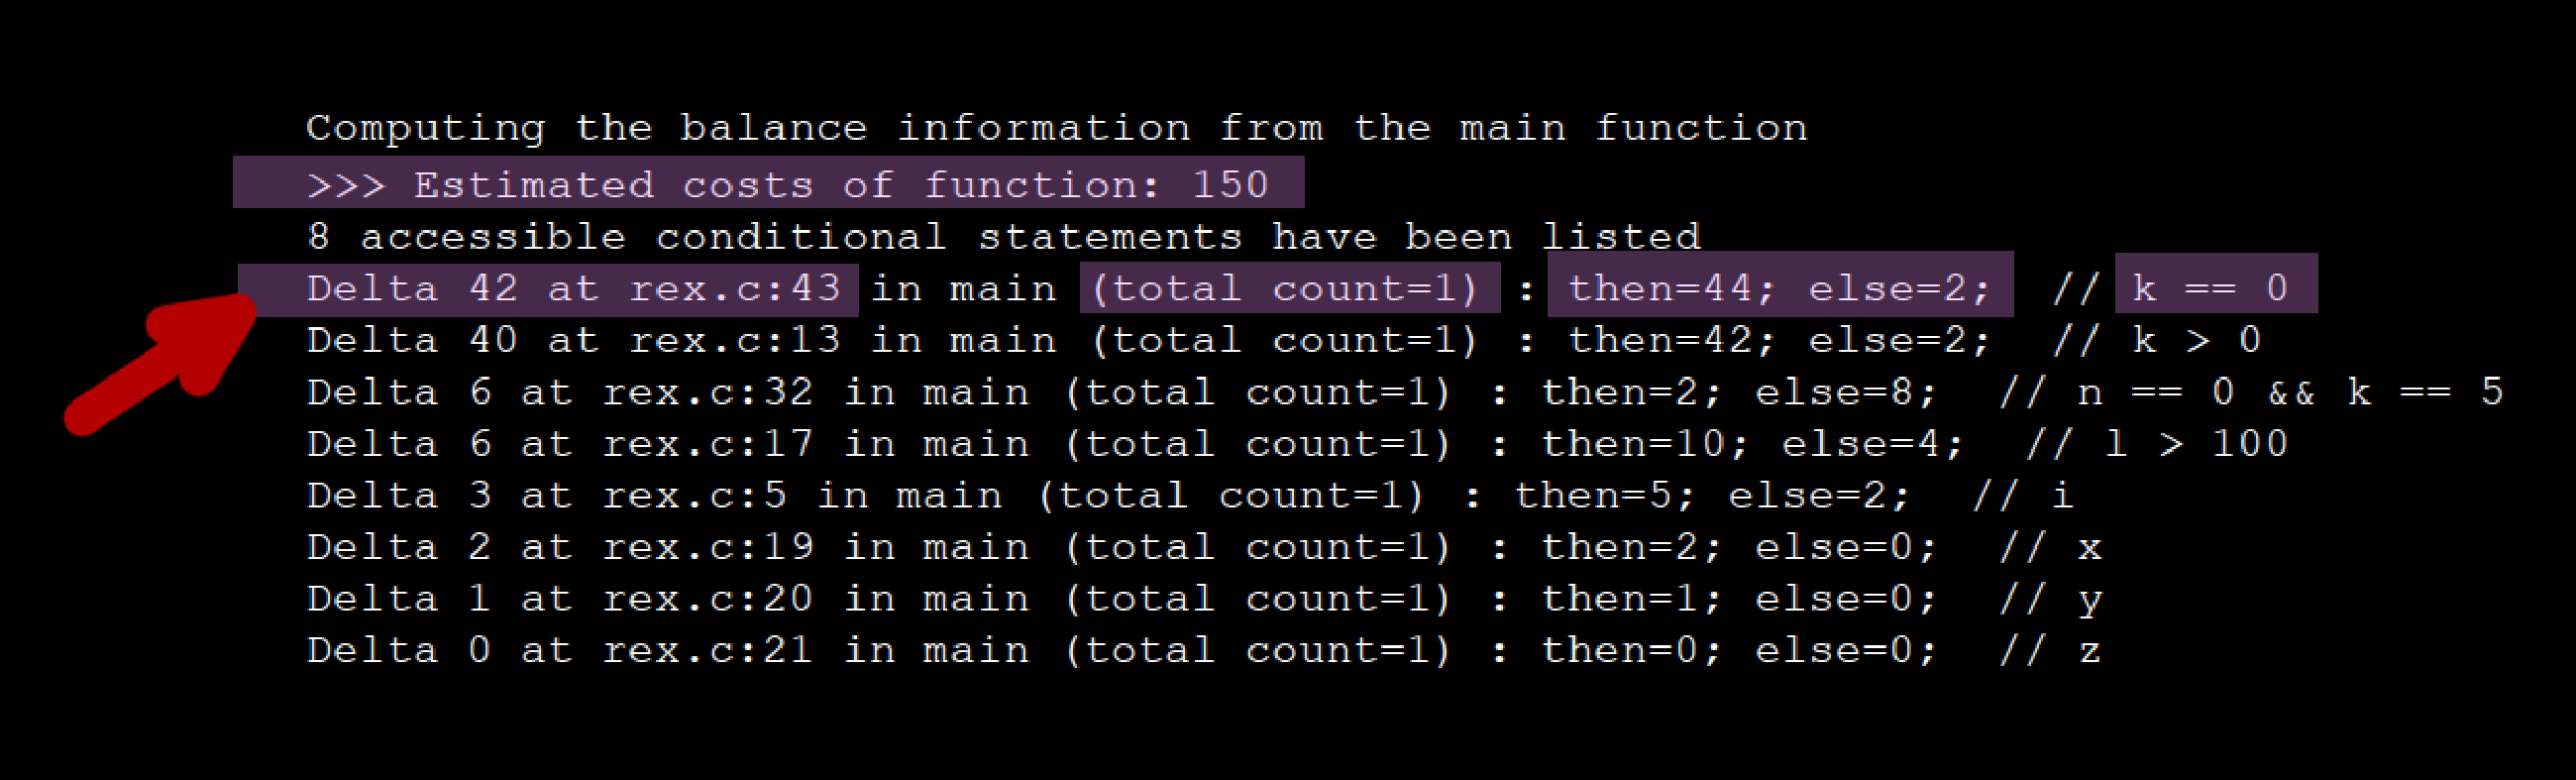
\includegraphics[width=9cm]{img/dd2.pdf} \\

    \bigskip
    Delta-weight and source location of a conditional.
  \end{center}
\end{frame} 
%%



% ---=== FRAME ===--- %
\begin{frame}[fragile]
  \frametitle{Delta Output: ``Normalized'' Costs}

  \begin{center}
    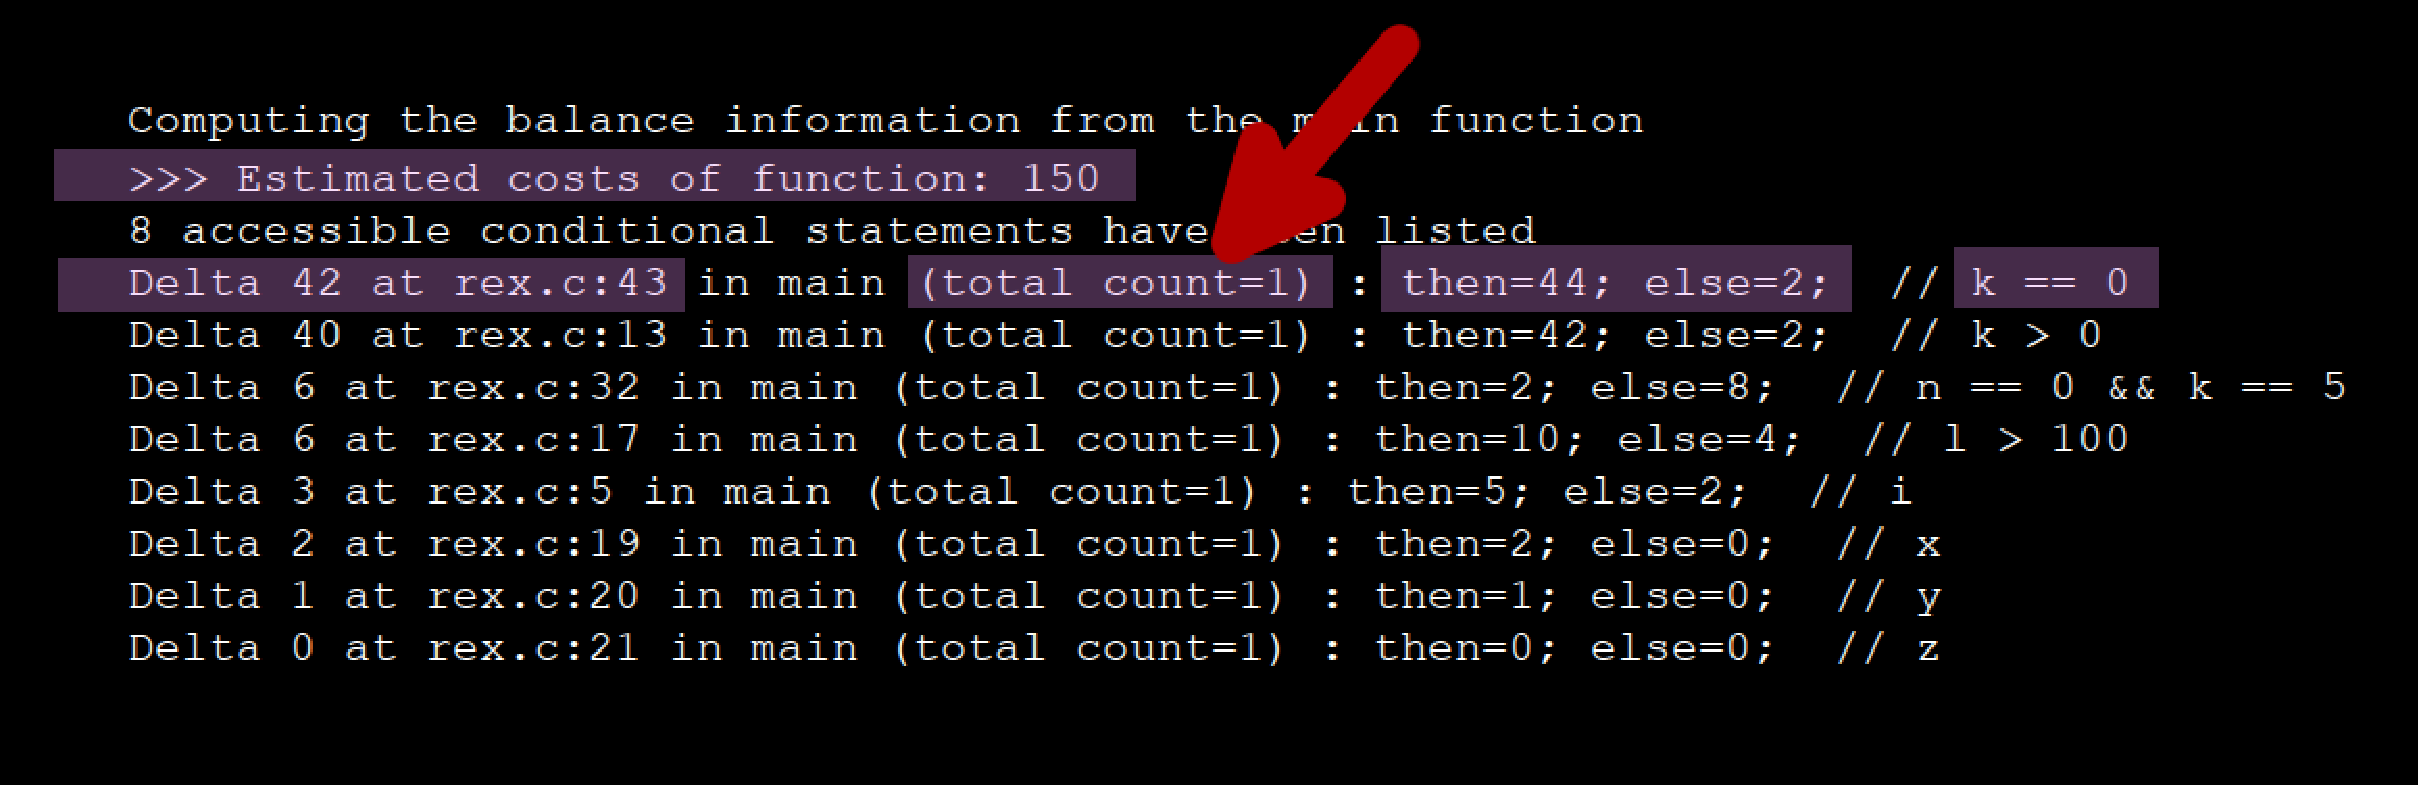
\includegraphics[width=9cm]{img/dd3.pdf} \\
  \end{center}

  \bigskip
  Delta-weight uses inferred information for weight-computation, i.e.
  \begin{itemize}
    \item loop bounds, $\mathit{weight}(n) \rightarrow  \mathit{weight}(n) * \ell$.
    \item infeasible paths $\mathit{executed}(n) = 0 \rightarrow \mathit{weight}(n) = 0$.
  \end{itemize}
\end{frame} 
%%



% ---=== FRAME ===--- %
\begin{frame}[fragile]
  \frametitle{Delta Output: Branch Weights}

  \begin{center}
    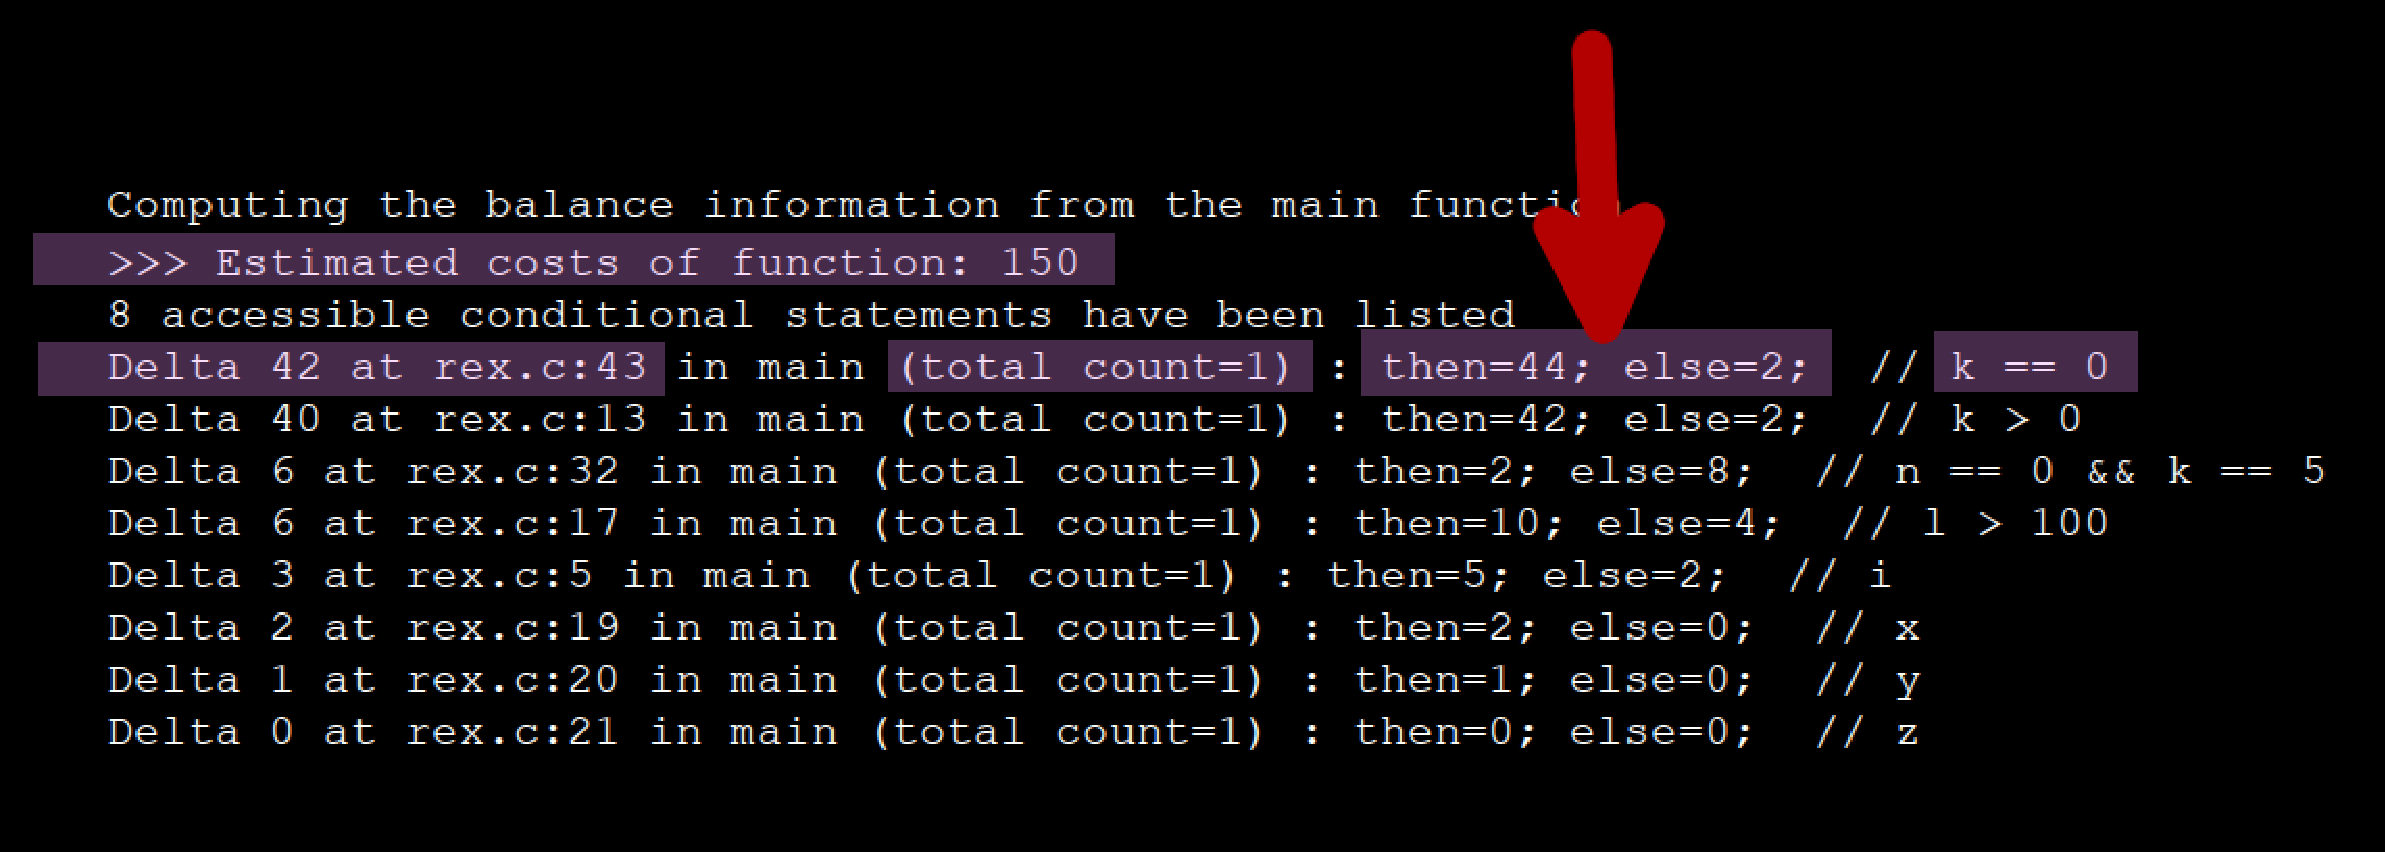
\includegraphics[width=9cm]{img/dd4.pdf} \\

    \bigskip
    Delta-weight of condition is computed from branch-weights. 
  \end{center}
\end{frame} 
%%



% ---=== FRAME ===--- %
\begin{frame}[fragile]
  \frametitle{Delta Output: Conditional Expression}

  \begin{center}
    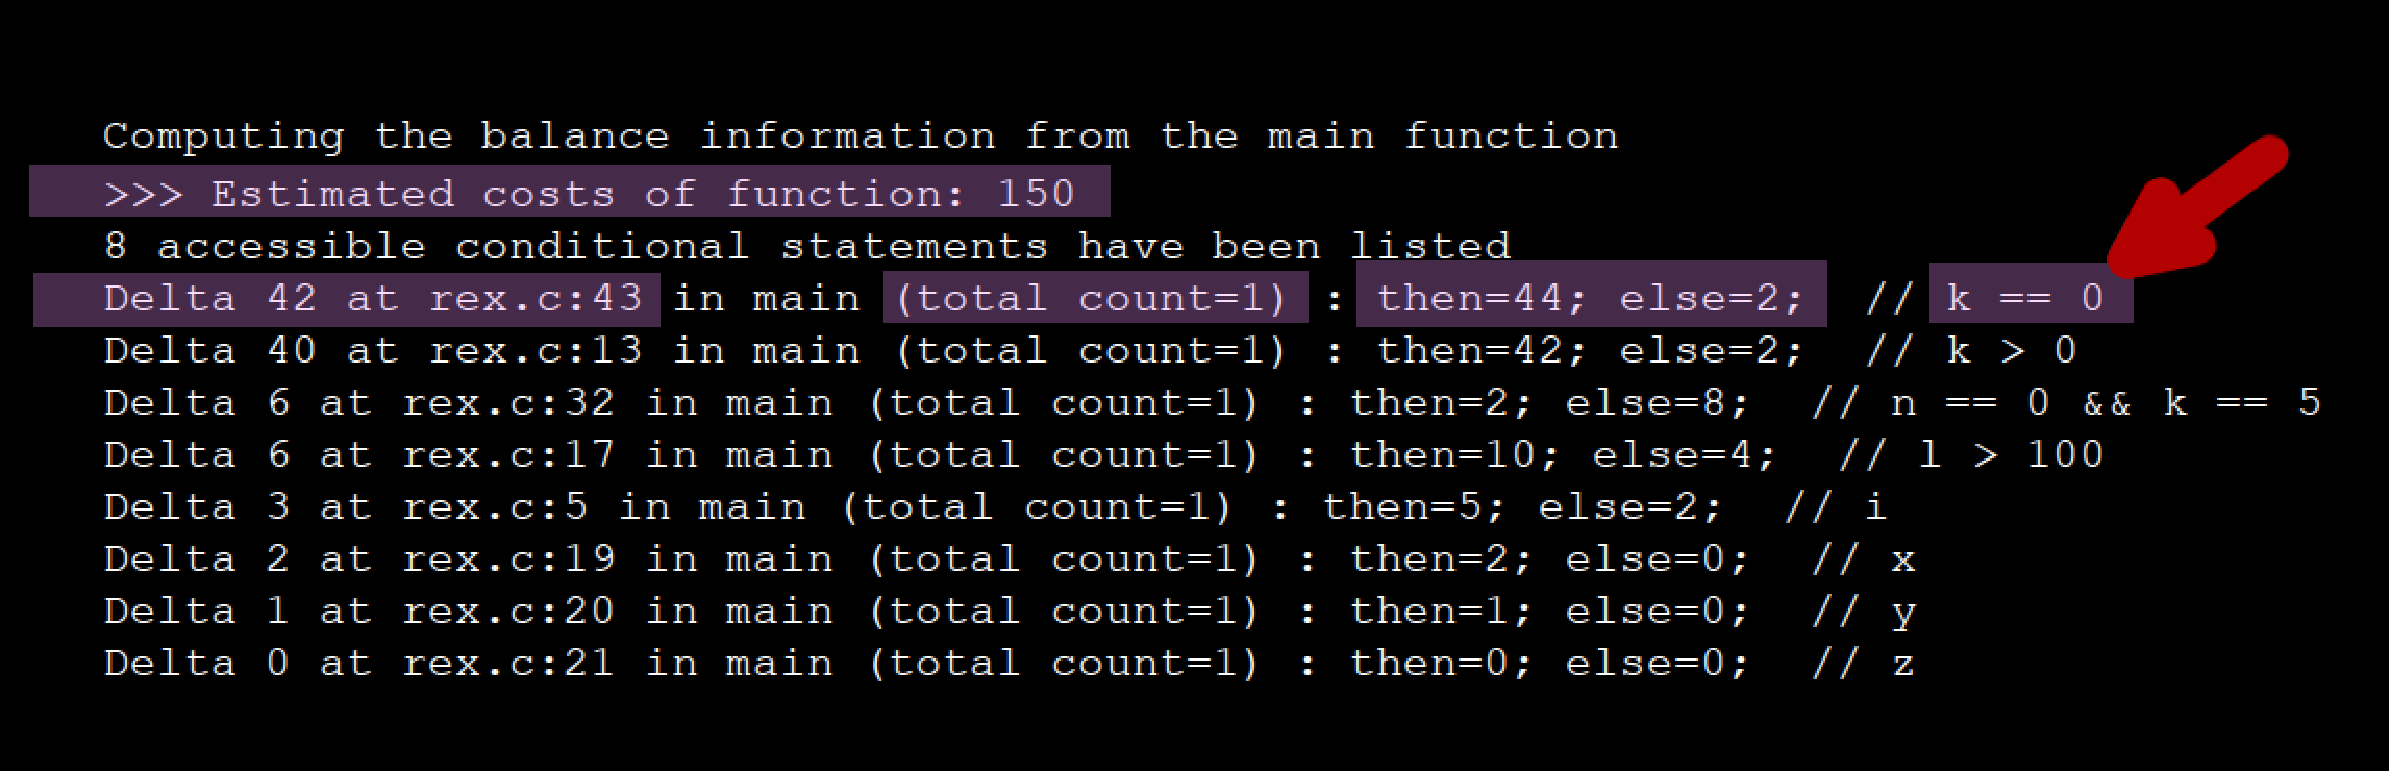
\includegraphics[width=9cm]{img/dd5.pdf} \\

    \bigskip
    (currently) strictly syntactic matching
  \end{center}
\end{frame} 
%%



% ---=== FRAME ===--- %
\begin{frame}[fragile]
  \frametitle{Now What, Why Do We Need That Again?}

  \bigskip
  Assume a program with overly high WCET estimate,
  \begin{itemize}
    \item a (huge) set of configuration variables, and a
    \item (huge) set of value restrictions for the configuration variables.
  \end{itemize}

  \pause 

  \bigskip
  Exhaustive specification is infeasible/tedious
  \begin{itemize}
    \item due to large set of configuration variables and ranges.
    \item (restrictions often {\bf unavailable}, not explicitly stated)
  \end{itemize}

  \bigskip
  :(
\end{frame} 
%%



% ---=== FRAME ===--- %
\begin{frame}[fragile]
  \frametitle{How Should Delta Analysis Help Again?}

  \bigskip
  Identifying relevant configuration variables is tedious,
  \begin{itemize}
    \item but automatic delta analysis can be used.
  \end{itemize}

  \bigskip
  Remember:
  \begin{itemize}
    \item high delta-weight $\leftrightarrow$ high impact on WCET
  \end{itemize}

  \pause

  \bigskip
  Relate high delta-weights to configuration variables
  \begin{itemize}
    \item and supply additional flow facts for those.
  \end{itemize}
\end{frame} 
%%



% ---=== FRAME ===--- %
\begin{frame}[fragile]
  \frametitle{Example: Continental Module}

  \bigskip
  Consists of
  \begin{itemize}
    \item {\tt an\_is.c}: the module
    \item {\tt missingFunctions.h}: missing function declarations 
    \item {\tt neededVariables.h}: parameter variable initializations
    \item (alternatively: an input FFX with value declarations)
  \end{itemize}

  \bigskip
  Additionally 
  \begin{itemize}
    \item set of 90 configuration/parameter variables
  \end{itemize}

  \bigskip
  Scenario, manually constructed and provided by expert
  \begin{itemize}
    \item 30 initial values for cfg/param variables
  \end{itemize}
\end{frame} 
%%



% ---=== FRAME ===--- %
\begin{frame}[fragile]
  \frametitle{Initial Analysis}

  \bigskip
  No scenario \\
  {\small 
  \begin{minted}{sh}
  > ./orange an_is_no_scenario/an_is.c main
  \end{minted}
  }
  \vspace{-.4cm}
  \begin{itemize}
    \item gives output FFX that can be supplied to OTAWA
  \end{itemize}

  \bigskip
  Full scenario \\
  {\small
  \begin{minted}{sh}
  > ./orange an_is_scenario/an_is.c main
  \end{minted}
  }
  \vspace{-.4cm}
  \begin{itemize}
    \item gives output FFX that can be supplied to OTAWA
    \item reports (hopefully) a tighter WCET estimate
  \end{itemize}

  \bigskip
  Scenario construction by an expert $\rightarrow$ tedious!
  \begin{itemize}
    \item delta analysis identifies relevant cfg/param variables
    \item less burden on developer (no need to manually choose 30)
  \end{itemize}
\end{frame}
%%



% ---=== FRAME ===--- %
\begin{frame}[fragile]
  \frametitle{Delta Analysis}

  \bigskip
  Apply delta analysis \\
  {\small
  \begin{minted}{sh}
  > ./orange an_is_no_scenario/an_is.c main --delta
  \end{minted}
  }
  \vspace{-.4cm}
  \begin{itemize}
    \item outputs the list of delta conditions
  \end{itemize}

  \bigskip
  Syntactic matching of cfg/param vars with vars in delta conditions 
  \begin{itemize}
    \item ``selects'' a number of {\bf relevant} cfg/param variables 
    \item specify initial values for only those
  \end{itemize}

  \bigskip
  $\Rightarrow$ smaller scenario, less effort to construct it
\end{frame} 
%%



% ---=== FRAME ===--- %
\begin{frame}[fragile]
  \frametitle{Delta Analysis Output}

  \bigskip
  {\tiny
  \begin{minted}{c}
>>> Estimated costs of function: 6907
51 accessible conditional statements have been listed
Delta 2034 at no_scenario/an_is.c:315 in c_n_sp_is (total count=1) : then=3; else=2037;  // lv_act_sa_eol
Delta 2034 at no_scenario/an_is.c:302 in c_n_sp_is (total count=1) : then=4; else=2038;  // lv_n_sp_is_lih_act
Delta 2033 at no_scenario/an_is.c:321 in c_n_sp_is (total count=1) : then=3; else=2036;  // lv_act_n_sp_is_ext_adj
Delta 2032 at no_scenario/an_is.c:327 in c_n_sp_is (total count=1) : then=3; else=2035;  // lv_act_n_sp_is_bas_ext_adj
Delta 230 at no_scenario/an_is.c:412 in c_n_dif (total count=1) : then=234; else=4;  // lv_is
Delta 218 at no_scenario/an_is.c:414 in c_n_dif (total count=1) : then=225; else=7;  // lv_n_dif_trans_is
Delta 215 at no_scenario/an_is.c:377 in c_n_sp_is (total count=1) : then=218; else=3;  // lv_st_end
Delta 184 at no_scenario/an_is.c:156 in c_n_sp_is (total count=1) : then=3; else=187;  // lv_var_acin
Delta 182 at no_scenario/an_is.c:162 in c_n_sp_is (total count=1) : then=2; else=184;  // tam < c_tam_n_sp_heat
Delta 16 at no_scenario/an_is.c:350 in c_n_sp_is (total count=1) : then=5; else=21;  // lv_n_sp_is_lih_act
Delta 11 at no_scenario/an_is.c:357 in c_n_sp_is (total count=1) : then=6; else=17;  // lv_n_sp_is_cs ? n_sp_is_3 == n_sp_is_cs : lv_n_sp_is_ramp_cs
Delta 10 at no_scenario/an_is.c:379 in c_n_sp_is (total count=1) : then=3; else=13;  // tmp_u32_n_sp_is_3_fine < n_sp_is_fine
Delta 8 at no_scenario/an_is.c:364 in c_n_sp_is (total count=1) : then=8; else=0;  // ((t_dly_n_sp_dec_pste ? n_sp_is_3 == n_sp_is_pste : lv_n_sp_is_ramp_pste)) || ((t_dly_n_sp_dec_pste_2 ? n_sp_is_3 == n_sp_is_pste_2 : lv_n_sp_is_ramp_pste_2))
Delta 8 at no_scenario/an_is.c:416 in c_n_dif (total count=1) : then=4; else=12;  // n_dif >= 0
Delta 8 at no_scenario/an_is.c:259 in c_n_sp_is (total count=1) : then=2; else=10;  // t_dly_n_sp_dec_pste
Delta 8 at no_scenario/an_is.c:287 in c_n_sp_is (total count=1) : then=2; else=10;  // t_dly_n_sp_dec_pste_2
Delta 5 at no_scenario/an_is.c:423 in c_n_dif (total count=1) : then=4; else=9;  // n_dif_3 >= n_dif
Delta 4 at no_scenario/an_is.c:275 in c_n_sp_is (total count=1) : then=9; else=13;  // 	((lv_pste_disable || lv_pste_2_disable || abs(ang_pste) > c_ang_pste_isc || abs(vel_ang_pste) > c_vel_ang_pste_isc)) && vs > c_vs_min_n_sp_pste_2
Delta 4 at no_scenario/an_is.c:248 in c_n_sp_is (total count=1) : then=9; else=13;  // 	lv_pste_disable || lv_pste_2_disable || lv_cs && !lv_var_amt || vs > c_vs_min_n_sp_pste || abs(ang_pste) > c_ang_pste_isc || abs(vel_ang_pste) > c_vel_ang_pste_isc
Delta 4 at no_scenario/an_is.c:450 in c_n_dif (total count=1) : then=2; else=6;  // n_dif_mmv > 0
Delta 3 at no_scenario/an_is.c:231 in c_n_sp_is (total count=1) : then=7; else=10;  // 	t_ast > t_ast_min_n_sp_is_cs && ((lv_is || lc_is_n_sp_cs_dis)) && lv_cs && !lv_var_amt && lv_cs_vs_in_hys
Delta 3 at no_scenario/an_is.c:430 in c_n_dif (total count=1) : then=5; else=2;  // lv_n_dif_crlc_marc || n_dif <= (int)((-150))
Delta 3 at no_scenario/an_is.c:456 in c_n_dif (total count=1) : then=3; else=0;  // n_dif_mmv < c_n_dif_min_mmv
Delta 3 at no_scenario/an_is.c:220 in c_n_sp_is (total count=1) : then=2; else=5;  // vs < u8_sub_u8_u8(c_vs_max_n_sp_cs, c_vs_hys_n_sp_cs)
Delta 3 at no_scenario/neededFunctions.h:18 in s16_min_max_s16_s16_s16 (total count=1) : then=6; else=9;  // value > maximum
Delta 3 at no_scenario/neededFunctions.h:65 in u8_sub_u8_u8 (total count=1) : then=8; else=5;  // x_value_0 > y_value_0
Delta 2 at no_scenario/an_is.c:240 in c_n_sp_is (total count=1) : then=2; else=0;  // !lv_n_sp_is_cs && lv_n_sp_is_ramp_end
Delta 2 at no_scenario/an_is.c:293 in c_n_sp_is (total count=1) : then=2; else=0;  // !lv_t_dly_pste_2_run && lv_n_sp_is_ramp_end
  \end{minted}
  }
\end{frame} 
%%



% ---=== FRAME ===--- %
\begin{frame}[fragile]
  \frametitle{Delta Analysis Result}

  \bigskip
  Pick highest 10 delta conditions (e.g.~delta10.txt) 
  {\small
  \begin{minted}{sh}
  > head -n 10 delta10.txt
  \end{minted}
  }

  \bigskip
  Syntactic matching on cfg/param variables \\
  \begin{itemize}
    \item to output the list of delta conditions.
  \end{itemize}

  \bigskip
  Currently, something like:
  {\small
  \begin{minted}{sh}
  > for var in `cut -d "," -f1 cfg_param_vars.csv`; 
    do 
      cut -d "/" -f 4 delta10.txt | grep -ow $var;
    done
  \end{minted}
  }

  \bigskip
  Could be a more complex (dependency) analyis 
\end{frame} 
%%



% ---=== FRAME ===--- %
\begin{frame}[fragile]
  \frametitle{Delta Scenario}

  \bigskip
  Selected variables
  {\tiny 
  \begin{minted}{sh}
c_tam_n_sp_heat, lv_act_n_sp_is_bas_ext_adj,
lv_act_n_sp_is_ext_adj, lv_act_sa_eol, lv_is,
lv_n_dif_trans_is, lv_n_sp_is_cs, lv_n_sp_is_lih_act,
lv_n_sp_is_lih_act, lv_n_sp_is_ramp_cs, lv_st_end,
lv_var_acin, n_sp_is_3, n_sp_is_cs, tam
  \end{minted}
  }

  \bigskip
  For those, initial values can be supplied via
  \begin{itemize}
    \item a header file ({\tt missingVariables.h})
    \item an input FFX file ({\tt in.ffx})
  \end{itemize}

  \bigskip
  Supplying initial values results in 18 infeasible paths
  {\small
  \begin{minted}{sh}
  > ./orange main an_is.c | grep executed=\"false | wc -l
  \end{minted}
  }
  \vspace{-.4cm}
  \begin{itemize}
    \item 18 ``not executed'' attributes set
  \end{itemize}
\end{frame}
%%


% ---=== FRAME ===--- %
\begin{frame}[fragile]
  \frametitle{Delta Scenario -- Input FFX}

  \bigskip
  As input FFX file:
  {\small
  \begin{minted}{sh}
  > ./orange main an_is.c --iffx in.ffx | 
                          grep executed=\"false | wc -l
  \end{minted}
  }

  \bigskip
  {\tt in.ffx}:
  {\tiny
  \begin{minted}{sh}
  <flowfacts>
     <context name="x">
        <data name="lv_act_sa_eol"><const value="0"/></data>
        <data name="lv_n_sp_is_lih_act"><const value="0"/></data>
        <data name="lv_is"><const value="1"/></data>
        <data name="lv_act_n_sp_is_ext_adj"><const value="0"/></data>
        <data name="lv_act_n_sp_is_bas_ext_adj"><const value="0"/></data>
        <data name="lv_st_end"><const value="1"/></data>
        <data name="lv_var_acin"><const value="0"/></data>
        <data name="tam"><const value="22"/></data>				
        <data name="c_tam_n_sp_heat"><const value="51"/></data>
        <data name="c_tam_hys"><const value="7"/></data>				
        <data name="lv_pste_disable"><const value="1"/></data>	
        <data name="vs"><const value="0"/></data>			
        <data name="lv_cs"><const value="0"/></data>		
        <data name="t_ast"><const value="0"/></data>	
        <data name="c_vs_max_n_sp_cs"><const value="10"/></data>	
        <data name="c_vs_hys_n_sp_cs"><const value="6"/></data>	
        <data name="lv_var_ars"><const value="0"/></data>		
        <data name="c_vs_min_n_sp_is_ars"><const value="0"/></data>
     </context>
  </flowfacts>
  \end{minted}
  }
\end{frame} 
%%



% ---=== FRAME ===--- %
\begin{frame}[fragile]
  \frametitle{Example -- {\tt hon.c}}
  {\tiny
  \begin{minipage}[t]{0.31\textwidth}
  \begin{minted}{c}
int expensive () {
  volatile int x, w;
  int y;
  return x + y * y + w * x;
}

int cheap () {
  volatile int x;
  return x;
}

int main (void) {
  volatile int p, q, r, s, t;
  int i, j, k;
  int init;

  if (init) {
    expensive(); 
  } else {
    cheap();
  }

  if (t < 10) {
    cheap();
  } else {
    expensive();
  }
  \end{minted}
  \end{minipage}
  \begin{minipage}[t]{0.32\textwidth}
  \begin{minted}{c}
  if (!r) {
    for (i = 0; i < 300; i++) 
      expensive();
  }

  for (i = 10; i < 100; i++) {
    if (t < i)        {
      expensive();
    }
    if (!init) {
      expensive();
    } else {
      cheap();
    }
  }
  if (p == 13) {
    for (j = 0; j < 10; j++) {
      if (q > 26) {
        expensive();
      } else {
        cheap();
      }
    }
  \end{minted}
  \end{minipage}
  \begin{minipage}[t]{0.32\textwidth}
  \begin{minted}{c}
  } else {
    if (r) {
      for (i = 0; i < 10; i++) {
        for (k = i; k < 10; k++) {
          if (s && t) {
            for (j = 0; j < 4; j++)
              expensive();
            } else {
              expensive();
          }
        }
      }
    } else {
      cheap();
    }
  } 
  return 0;
}
  \end{minted}
  \end{minipage}
  }
\end{frame}



% ---=== FRAME ===--- %
\begin{frame}[fragile]
  \frametitle{Experiments}
  \textcolor{red}{BEWARE: some of the techniques below can not be applied with a WCET analyzer}
  Answer the following questions, watch changes in delta condition weights after each step.
  \begin{enumerate}
    \item run delta analysis on {\tt hon.c} and interpret the output.
    \item how many of the resulting delta conditions should be considered? 
    \item analyze the costs of the function considering both phases of the most expensive delta cond.
    \item same for the 2nd highest delta cond.
    \item what value range of {\tt t} will further reduce the estimate?
    \item analyze the program in mode {\tt init} and {\tt !init}, extending the input ffx generated so far.
    \item what is the cost of {\tt expensive} and {\tt cheap} and how to get it?
  \end{enumerate}
\end{frame}
%%



% ---=== FRAME ===--- %
\begin{frame}[fragile]
  \frametitle{Solution 1}
  {\small
  \begin{minted}{sh}
    > ./orange main hon.c --delta
  \end{minted}
  }
  {\tiny
  \begin{minted}{sh}
>>> Estimated costs of function: 13604
9 accessible conditional statements have been listed
Delta 6570 at hon/hon.c:80 in main (total count=1) : then=6574; else=4;  // r
Delta 6411 at hon/hon.c:64 in main (total count=1) : then=164; else=6575;  // p == 13
Delta 4800 at hon/hon.c:86 in main (total count=100) : then=60; else=12;  // s && t
Delta 4204 at hon/hon.c:42 in main (total count=1) : then=4204; else=0;  // !r
Delta 1080 at hon/hon.c:50 in main (total count=90) : then=12; else=0;  // t < i
Delta 720 at hon/hon.c:54 in main (total count=90) : then=12; else=4;  // !init
Delta 80 at hon/hon.c:68 in main (total count=10) : then=12; else=4;  // q > 26
Delta 8 at hon/hon.c:33 in main (total count=1) : then=4; else=12;  // t < 10
Delta 8 at hon/hon.c:24 in main (total count=1) : then=12; else=4;  // init
  \end{minted}
  }
\end{frame}



% ---=== FRAME ===--- %
\begin{frame}[fragile]
  \frametitle{Solution 2}
  It's 9 deltas, costs of function is 13604. \\
  6 highest deltas cost 6570 to 720, those should make sense.
\end{frame}



% ---=== FRAME ===--- %
\begin{frame}[fragile]
  \frametitle{Solution 3}
  Use input 3.ffx, setting the value of r == 1, this gives the cost for the other (cheaper) phase.
  {\small
  \begin{minted}{xml}
<flowfacts>
  <context name="p3">
    <data name="r"><const value="1"/></data>
  </context>
</flowfacts>
  \end{minted}
  }
  finds infeasible path: line 44, line 100, costs: 9400 
  {\small
  \begin{minted}{sh}
    > ./orange main hon.c --delta --iffx 3.ffx
  \end{minted}
  }
\end{frame}
%% 



% ---=== FRAME ===--- %
\begin{frame}[fragile]
  \frametitle{Solution 4}
  Use input 4.ffx, setting the value of r == 1 and p == 13,
  this gives the cost for the other (cheaper) phase.
  {\small
  \begin{minted}{xml}
<flowfacts>
  <context name="p4">
    <data name="r"><const value="1"/></data>
    <data name="p"><const value="13"/></data>
  </context>
</flowfacts>
  \end{minted}
  }
  Finds infeasible path: line 44, line 100, line 80, costs: 2989
  {\small
  \begin{minted}{sh}
    > ./orange main hon.c --delta --iffx 4.ffx
  \end{minted}
  }
\end{frame}
%%



% ---=== FRAME ===--- %
\begin{frame}[fragile]
  \frametitle{Solution 5}
  If {\tt t} is less than 10, the estimate is lower: even though it disables
  the ``locally'' cheaper path through the else branch of the cond in line 33,
  the piece in the loop is ``globally'' more expensive (if {\tt t < 10}).
  {\small
  \begin{minted}{xml}
<flowfacts>
  <context name="p5">
    <data name="r"><const value="1"/></data>
    <data name="p"><const value="13"/></data>
    <data name="t"><const value="0"/></data>
  </context>
</flowfacts>
  \end{minted}
  }
  finds infeasible path: line 44, line 100, line 80, line 39, costs: 2981.
  {\small
  \begin{minted}{sh}
    > ./orange main hon.c --delta --iffx 5.ffx
  \end{minted}
  }
\end{frame}
%%



% ---=== FRAME ===--- %
\begin{frame}[fragile]
  \frametitle{Solution 6}
  Specify {\tt init == 0} and {\tt init != 0} in the ffx. (DON'T do this with other analyzers)
  {\small
  \begin{minted}{xml}
<flowfacts>
  <context name="p61">
    <data name="r"><const value="1"/></data>
    <data name="p"><const value="13"/></data>
    <data name="t"><const value="0"/></data>
    <data name="init"><const value="0"/></data>
  </context>
</flowfacts>

<flowfacts>
  <context name="p62">
    <data name="r"><const value="1"/></data>
    <data name="p"><const value="13"/></data>
    <data name="t"><const value="0"/></data>
    <data name="init"><const value="1"/></data>
  </context>
</flowfacts>  
  \end{minted}
  }
  costs when {\tt init}: 2981 \\
  costs when {\tt !init}: 2973
  {\small
  \begin{minted}{sh}
    > ./orange main hon.c --delta --iffx 61.ffx
    > ./orange main hon.c --delta --iffx 62.ffx
  \end{minted}
  }
\end{frame}
%%



% ---=== FRAME ===--- %
\begin{frame}[fragile]
  \frametitle{Solution 7}
  As we currently support analyzing the main function only, the solution is to 
  put the two function into seperate C files, renaming them to {\tt main} and then
  running the analysis. \\
  costs of {\tt expensive}: 12 \\
  costs of {\tt cheap}: 4 \\
\end{frame}


%numitor
%topcased


\end{document}
